\documentclass[a4paper,12pt,twoside]{memoir}

% Castellano
\usepackage[spanish,es-tabla]{babel}
\selectlanguage{spanish}
\usepackage[utf8]{inputenc}
\usepackage[T1]{fontenc}
\usepackage{lmodern} % scalable font
\usepackage{microtype}
\usepackage{placeins}


\RequirePackage{booktabs}
\RequirePackage[table]{xcolor}
\RequirePackage{xtab}
\RequirePackage{multirow}

% Links
\usepackage[colorlinks]{hyperref}
\hypersetup{
	allcolors = {red}
}

% Ecuaciones
\usepackage{amsmath}

% Rutas de fichero / paquete
\newcommand{\ruta}[1]{{\sffamily #1}}

% Párrafos
\nonzeroparskip


% Imagenes
\usepackage{graphicx}
\usepackage{wrapfig}
\newcommand{\imagen}[2]{
	\begin{figure}[!h]
		\centering
		\includegraphics[width=0.9\textwidth]{#1}
		\caption{#2}\label{fig:#1}
	\end{figure}
	\FloatBarrier
}

\newcommand{\imagenflotante}[2]{
	\begin{figure}%[!h]
		\centering
		\includegraphics[width=0.9\textwidth]{#1}
		\caption{#2}\label{fig:#1}
	\end{figure}
}



% El comando \figura nos permite insertar figuras comodamente, y utilizando
% siempre el mismo formato. Los parametros son:
% 1 -> Porcentaje del ancho de página que ocupará la figura (de 0 a 1)
% 2 --> Fichero de la imagen
% 3 --> Texto a pie de imagen
% 4 --> Etiqueta (label) para referencias
% 5 --> Opciones que queramos pasarle al \includegraphics
% 6 --> Opciones de posicionamiento a pasarle a \begin{figure}
\newcommand{\figuraConPosicion}[6]{%
  \setlength{\anchoFloat}{#1\textwidth}%
  \addtolength{\anchoFloat}{-4\fboxsep}%
  \setlength{\anchoFigura}{\anchoFloat}%
  \begin{figure}[#6]
    \begin{center}%
      \Ovalbox{%
        \begin{minipage}{\anchoFloat}%
          \begin{center}%
            \includegraphics[width=\anchoFigura,#5]{#2}%
            \caption{#3}%
            \label{#4}%
          \end{center}%
        \end{minipage}
      }%
    \end{center}%
  \end{figure}%
}

%
% Comando para incluir imágenes en formato apaisado (sin marco).
\newcommand{\figuraApaisadaSinMarco}[5]{%
  \begin{figure}%
    \begin{center}%
    \includegraphics[angle=90,height=#1\textheight,#5]{#2}%
    \caption{#3}%
    \label{#4}%
    \end{center}%
  \end{figure}%
}
% Para las tablas
\newcommand{\otoprule}{\midrule [\heavyrulewidth]}
%
% Nuevo comando para tablas pequeñas (menos de una página).
\newcommand{\tablaSmall}[5]{%
 \begin{table}
  \begin{center}
   \rowcolors {2}{gray!35}{}
   \begin{tabular}{#2}
    \toprule
    #4
    \otoprule
    #5
    \bottomrule
   \end{tabular}
   \caption{#1}
   \label{tabla:#3}
  \end{center}
 \end{table}
}

%
%Para el float H de tablaSmallSinColores
\usepackage{float}

%
% Nuevo comando para tablas pequeñas (menos de una página).
\newcommand{\tablaSmallSinColores}[5]{%
 \begin{table}[H]
  \begin{center}
   \begin{tabular}{#2}
    \toprule
    #4
    \otoprule
    #5
    \bottomrule
   \end{tabular}
   \caption{#1}
   \label{tabla:#3}
  \end{center}
 \end{table}
}

\newcommand{\tablaApaisadaSmall}[5]{%
\begin{landscape}
  \begin{table}
   \begin{center}
    \rowcolors {2}{gray!35}{}
    \begin{tabular}{#2}
     \toprule
     #4
     \otoprule
     #5
     \bottomrule
    \end{tabular}
    \caption{#1}
    \label{tabla:#3}
   \end{center}
  \end{table}
\end{landscape}
}

%
% Nuevo comando para tablas grandes con cabecera y filas alternas coloreadas en gris.
\newcommand{\tabla}[6]{%
  \begin{center}
    \tablefirsthead{
      \toprule
      #5
      \otoprule
    }
    \tablehead{
      \multicolumn{#3}{l}{\small\sl continúa desde la página anterior}\\
      \toprule
      #5
      \otoprule
    }
    \tabletail{
      \hline
      \multicolumn{#3}{r}{\small\sl continúa en la página siguiente}\\
    }
    \tablelasttail{
      \hline
    }
    \bottomcaption{#1}
    \rowcolors {2}{gray!35}{}
    \begin{xtabular}{#2}
      #6
      \bottomrule
    \end{xtabular}
    \label{tabla:#4}
  \end{center}
}

%
% Nuevo comando para tablas grandes con cabecera.
\newcommand{\tablaSinColores}[6]{%
  \begin{center}
    \tablefirsthead{
      \toprule
      #5
      \otoprule
    }
    \tablehead{
      \multicolumn{#3}{l}{\small\sl continúa desde la página anterior}\\
      \toprule
      #5
      \otoprule
    }
    \tabletail{
      \hline
      \multicolumn{#3}{r}{\small\sl continúa en la página siguiente}\\
    }
    \tablelasttail{
      \hline
    }
    \bottomcaption{#1}
    \begin{xtabular}{#2}
      #6
      \bottomrule
    \end{xtabular}
    \label{tabla:#4}
  \end{center}
}

%
% Nuevo comando para tablas grandes sin cabecera.
\newcommand{\tablaSinCabecera}[5]{%
  \begin{center}
    \tablefirsthead{
      \toprule
    }
    \tablehead{
      \multicolumn{#3}{l}{\small\sl continúa desde la página anterior}\\
      \hline
    }
    \tabletail{
      \hline
      \multicolumn{#3}{r}{\small\sl continúa en la página siguiente}\\
    }
    \tablelasttail{
      \hline
    }
    \bottomcaption{#1}
  \begin{xtabular}{#2}
    #5
   \bottomrule
  \end{xtabular}
  \label{tabla:#4}
  \end{center}
}



\definecolor{cgoLight}{HTML}{EEEEEE}
\definecolor{cgoExtralight}{HTML}{FFFFFF}

%
% Nuevo comando para tablas grandes sin cabecera.
\newcommand{\tablaSinCabeceraConBandas}[5]{%
  \begin{center}
    \tablefirsthead{
      \toprule
    }
    \tablehead{
      \multicolumn{#3}{l}{\small\sl continúa desde la página anterior}\\
      \hline
    }
    \tabletail{
      \hline
      \multicolumn{#3}{r}{\small\sl continúa en la página siguiente}\\
    }
    \tablelasttail{
      \hline
    }
    \bottomcaption{#1}
    \rowcolors[]{1}{cgoExtralight}{cgoLight}

  \begin{xtabular}{#2}
    #5
   \bottomrule
  \end{xtabular}
  \label{tabla:#4}
  \end{center}
}




\graphicspath{ {./img/} }

% Capítulos
\chapterstyle{bianchi}
\newcommand{\capitulo}[2]{
	\setcounter{chapter}{#1}
	\setcounter{section}{0}
	\chapter*{#2}
	\addcontentsline{toc}{chapter}{#2}
	\markboth{#2}{#2}
}

% Apéndices
\renewcommand{\appendixname}{Apéndice}
\renewcommand*\cftappendixname{\appendixname}

\newcommand{\apendice}[1]{
	%\renewcommand{\thechapter}{A}
	\chapter{#1}
}

\renewcommand*\cftappendixname{\appendixname\ }

% Formato de portada
\makeatletter
\usepackage{xcolor}
\newcommand{\tutor}[1]{\def\@tutor{#1}}
\newcommand{\course}[1]{\def\@course{#1}}
\definecolor{cpardoBox}{HTML}{E6E6FF}
\def\maketitle{
  \null
  \thispagestyle{empty}
  % Cabecera ----------------
\noindent
\includegraphics[width=\textwidth]{cabecera}\vspace{1cm}%
  \vfill
  % Título proyecto y escudo informática ----------------
  \colorbox{cpardoBox}{%
    \begin{minipage}{.8\textwidth}
      \vspace{.5cm}\Large
      \begin{center}
      \textbf{TFG del Grado en Ingeniería Informática}\vspace{.6cm}\\
      \textbf{\LARGE\@title{}}
      \end{center}
      \vspace{.2cm}
    \end{minipage}

  }%
  \hfill\begin{minipage}{.20\textwidth}
    
\includegraphics[width=\textwidth]{escudoInfor}
  \end{minipage}
  \vfill
  % Datos de alumno, curso y tutores ------------------
  \begin{center}%
  {%
    \noindent\LARGE
    Presentado por \@author{}\\ 
    en Universidad de Burgos --- \@date{}\\
    \@tutor{}\\
  }%
  \end{center}%
  \null
  \cleardoublepage
  }
\makeatother


% Datos de portada
\title{Aplicación de tecnología Blockchain a una cadena de distribución de productoser \\Documentación Técnica}
\author{Eduardo Rodríguez Soto}
\tutor{Tutor académico: Ángel Arroyo Puente\\
Tutor empresarial en HP: Pablo Tejedor García}
\date{\today}

\begin{document}

\maketitle

\cleardoublepage


%%%%%%%%%%%%%%%%%%%%%%%%%%%%%%%%%%%%%%%%%%%%%%%%%%%%%%%%%%%%%%%%%%%%%%%%%%%%%%%%%%%%%%%%


\frontmatter


\clearpage

% Indices
\tableofcontents

\clearpage

\listoffigures

\clearpage

\listoftables

\clearpage

\mainmatter

\appendix

\apendice{Plan de Proyecto Software}

\section{Introducción}

Cuando queremos hablar de la realización de proyecto, nos encontramos con una fase primordial, que es es la planificación. En esta etapa se estiman los tiempos y el presupuesto del proyecto. 

Para hablar de estas estimaciones, se debe tener en cuenta las partes que realizan el proyecto estén de acuerdo con todas las ideas planteadas. Se dividirán en dos partes: 

\begin{itemize}
	\item \textit{Planificación temporal}: hablaremos de todas las reuniones realizadas y además comprobaremos si los tiempos de la realización del proyecto son óptimos.
	\item \textit{Estudio de viabilidad}: intentaremos decidir si el proyecto fue bien planteado o falló algo en la ejecución, dentro de este estudio, tendremos dos tipos de viabilidad:
	\begin{enumerate}[a]
		\item \textit{Económica}: explicaremos los costes y posibles beneficios del proyecto.
		\item \textit{Legal}: estudiaremos las leyes que tuvieran que ver con nuestro proyecto.
	\end{enumerate}
\end{itemize}

\section{Planificación temporal}

Como hablamos en la memoria, utilizaremos una metodología Scrum. Las características de este método son:

\begin{itemize}
	\item Utilizaremos una estrategia de sprint para esta metodología, dividiremos el trabajo en intervalos de un tiempo y así observaremos su desarrollo.
	\item Con cada sprint se planifican las tareas a realizar y el tiempo en el que desarrollaremos el trabajo. En general las reuniones fueron cada dos semanas.
	\item Al finalizar el sprint, realizaremos una reunión mediante videollamada o asistiendo personalmente a León.
\end{itemize}

El inicio del proyecto comienza con una reunión con el tutor Pablo Tejedor García mediante una llamada telefónica, en ella hablamos un poco acerca del porqué de la elección de este trabajo y cuales serán los objetivos del proyecto y las opciones que tendremos para realizarlas. 

El tutor de HP, me comentó que es un proyecto de investigación,  con una tecnológica nunca utilizada anteriormente en dicha empresa, el mundo Blockchain.


\subsection{Sprint 1 (24/10/18 - 16/11/18)}

En la primera reunión realizada hablamos de los objetivos y la realización de la siguiente tarea:

\begin{itemize}
	\item Lectura del libro \textit{``Scrum desde las trincheras''} \cite{libro}.
	\item Realización del curso ``CrytoZombies''.
\end{itemize}

Se calculan 30 horas de trabajo.

\subsection{Sprint 2 (16/11/18 - 15/01/19)}

Primeramente hablamos de la conclusión del sprint anterior y cómo fue la primera toma de contacto con un lenguaje nunca usado anteriormente.

Para esta segunda reunión se propusieron las siguientes tareas:
\begin{itemize}
	\item Resumen del libro leído en el sprint anterior.
	\item Creación de un \textit{smart contract}, con cierta funcionalidad en modo local.
	\item Realización de programas en Visual Studio, para la realización de pequeños archivos.
	\item Investigación de Truffle como entorno, ya que es una plataforma que nos permitirá desarrollar \textit{smart contracts} y desplegarlos para poder consumirlos desde un frontEnd.
\end{itemize}

Se calculan 45 horas de trabajo.

\subsection{Sprint 3 (15/01/19 - 12/02/19)}

Para esta nueva tarea se proponen las siguientes tareas:

\begin{itemize}
	\item Documentación somera de Truffle. Necesitamos una pequeña guía de que es, cómo instalarlo y qué funcionalidades proporciona Truffle para la memoria del Proyecto.
	\item Desarrollo de un \textit{smart contract} sencillo con la plataforma Truffle. Un pequeño \textit{smart contract} funcional con el que podamos empezar a trabajar.
	\item Desarrollo de una pequeña aplicación de escritorio o web (a decisión del alumno) en Visual Studio 2017 que disponga de una sola pantalla y elementos para interactuar con la capa de abajo donde se situará el \textit{smart contract} desplegado.
\end{itemize}

Se calculan 40 horas de trabajo.

\subsection{Sprint 4 (12/02/19 - 28/02/19)}

Para la cuarta reunión en el proyecto se habló de la sesión anterior, en la cual comprobamos el guión de Truffle. Realizamos la ejecución de los \textit{smart contract} realizados en el lenguaje Solidity y visualización de los proyectos creados en la aplicación Visual Studio 2017.

Las tareas a realizar para la siguiente sesión serán: 

\begin{itemize}
	\item Realización de un guión con la información a poner en la memoria.
	\item Investigación sobre web3.js (conexión entre Visual Studio y Ethereum).
	\item Creación de página de autobuses para realizar un simulacro de la página final, pero con modo local (Ganache).
\end{itemize}

Se calculan 52 horas de trabajo.

\subsection{Sprint 5 (28/02/19 - 29/03/19)}

Comentamos los problemas que surgieron en la sprint 4.

El principal quebradero de cabeza del sprint anterior fue la conexión entre web3.js, no sabíamos dar con el error ya que cuando probamos la aplicación nueva de autobuses con Ganache (modo Local) la conexión era perfecta y realizaba el cambio de divisa sin ningún problema.

Intentamos buscar alternativas cuando teníamos el error con web3.js (en modo red privada global o red principal Ethereum). Me propuso realizar la aplicación olvidándonos de la conexión con Ethereum y realizar una base de datos para poder mostrar todo desde ahí.

Pero seguimos indagando e intentamos realizarlo, pero con otras propuestas de editores de código.

\begin{itemize}
	\item Realizar conexión entre metamask y un editor de código, con web3.
	\item Desarrollar el guión creado del sprint anterior.
\end{itemize}

Se calculan 25 horas de trabajo.

\subsection{Sprint 6 (29/03/19 - 08/04/19)}

Esta reunión se realizo en León de forma presencial y en ella comentamos el guion y la posibilidad de modificar algún punto para la mayor compresión de esta nueva tecnología.

Expliqué a Pablo el editor nuevo usado para la conexión de Ethereum y nuestro editor, y conseguimos la conexión entre ambos medios; pudiendo así realizar los \textit{smart contract}, tanto en red local, privada y global (esto lo conseguimos en Visual Stuido Code).

Una vez teníamos la conexión realizada ya teníamos una gran parte del objetivo del proyecto realizado.

Los siguientes objetivos a tratar para hablar de ellos en el siguiente sprint fueron:

\begin{itemize}
	\item Creación de la pagina web, con las diferentes pantallas y la conexión entre ellas que fuera correctas.
	\item Buscar una base de datos para nuestro proyecto. 
	\item Documentar la memoria.
\end{itemize}

Se calculan 60 horas de trabajo.
	
\subsection{Sprint 7 (08/04/19 - 02/05/19)}

Comentamos las páginas creadas de nuestra web, comprobamos la funcionalidad con metamask y este con Ethereum. La conexión era buena, ahora queda realizar los css y dejar la página armonizar todas las páginas. 

La base de datos que realizamos es la de MySql, se encarga de almacenar a los usuarios y los datos enviados a la red Ethereum.

Para el siguiente sprint los objetivos serían:

\begin{itemize}
	\item Armonización de la página web en todas sus páginas.
	\item Creación de página de Administrador que pueda manejar a todos los usuarios que tenemos registrados.
	\item Poder seleccionar un avatar cuando creamos usuario.
\end{itemize}

Se calculan 27 horas de trabajo.


\subsection{Parón de los Sprint (02/05/19 - 23/10/19)}

En esta reunión comente la idea de que me iba de viaje a Estados Unidos y la fecha de ir no sería posible la entrega del Tfg de modo presencia, y que era demasiado tarde para poder cambiarlo a modo on-line, les hable de mi idea de continuar con el mismo Tfg para entregar en la primera convocatoria del curso 2019/2020.

Lo que supuso que en este parón hasta volver de Estados Unidos no realizaramos ningún Sprint ni hubiera avances en el desarrollo del proyecto.


\subsection{Sprint 8 (23/10/19 - 18/11/19)}

En esta reunión hablamos sobre pequeñas funcionalidades de nuestra página que se podrían añadir:

\begin{itemize}
	\item Introducción de un código \textit{captha} cuando se registra el usuario.
	\item Creación de una nueva página: ¿Has olvidado la contraseña?
	\item Modificación de la visualización de todos los productos pedidos.
	\item Comenzar con el apartado de los anexos, explicación de cada sprint.
\end{itemize}

También nos dimos cuenta de que la red Ropsten se nos estaba quedando sin Ether y pensamos en suprimir el dinero cada vez que se realiza el \textit{smart contract} y dejar solamente el gas de cada transacción.

Se calculan 45 horas de trabajo.

\subsection{Sprint 9 (18/11/19 - 12/12/19)}

Primeramente hablamos de la reunión anterior y comentamos la dificultad encontrada en realizar la función del \textit{captha} y ¿Has olvidado la contraseña?, ya que al ser en modo local y no tener un dominio, tendríamos que realizarlo de otras maneras.

El objetivo para la décima reunión es:

\begin{itemize}
	\item Mejorar los apartados resumen, introducción y concretos teóricos de la memoria.
	\item Investigar la opción de realizar el captha y ¿has olvidado la contraseña? mediante otro método.
	\item Continuar con los anexos.
\end{itemize}

Se calculan 37 horas de trabajo.


\subsection{Sprint 10 (12/12/19 - 20/12/2019)}

En la décima reunión hablamos de lo siguiente:

\begin{itemize}
	\item Finalizar de la página Web.
	\item Intentar crear un ejecutable para nuestra aplicación.
	\item Finalizar la memoria y anexos.
\end{itemize}

Se calculan 55 horas de trabajo.

\subsection{Sprint 11 (20/12/2019 - entrega proyecto)}

En la última reunión hablamos de lo siguiente:

\begin{itemize}
	\item Comprobar todas la funcionalidad de la web y la conexión con la red Ethereum.
	\item Decisión de realizar la entrega desde la cuenta Localhost.
	\item Revisar la memoria y anexos.
	\item Descargar todos los documentos para visualizar la información y ver que es correcta. Así evitaremos que se pueda encontrar imágenes cortadas o textos mal indexados.
\end{itemize}


\subsection{Resumen}

En la siguiente tabla \ref{tabla:tabla1}, veremos la distribución del tiempo en las diferentes tareas que se realizarón  para la elaboración de este proyecto, cada tarea se expresa en horas:

\begin{table}[H]
	\begin{center}
		\begin{tabular}{|l|l|}
		\hline
			Tarea a realizar & Tiempo(horas)\\ 
			\hline \hline
			Programación & 150 \\ \hline
			Investigación & 105 \\ \hline
			Documentación & 90 \\ \hline
			Revisión y corrección de errores & 54\\ \hline
			Reuniones & 17 \\ \hline
			Total & 416 \\ \hline
		\end{tabular}
	\caption{Tiempo empleado en el proyecto.}
	\label{tabla:tabla1}
	\end{center}
\end{table}

En el siguiente gráfico \ref{ref:horas}, observaremos el tiempo empleado estructurado en el desarrollo del proyecto.

\begin{figure}
    \centering
    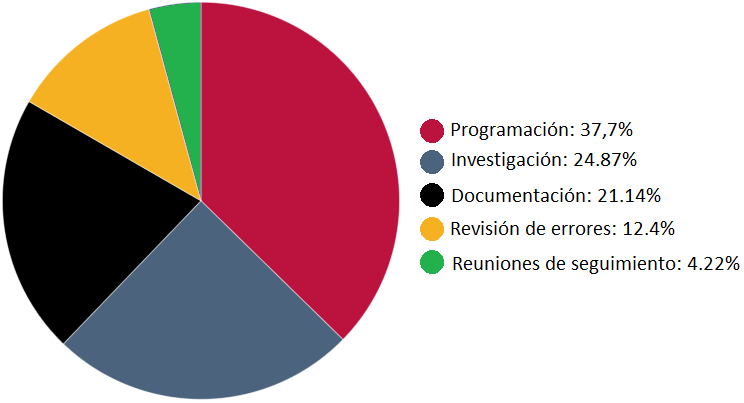
\includegraphics[width=0.80\textwidth]{quesitoTiempo}
    \caption{Gráfico de las horas empleadas en el proyecto}
    \label{ref:horas}
\end{figure}
 
A continuación explicaremos, el proceso de los sprint con una breve explicación de las tareas que se realizan en cada una de ellas \ref{tabla:sprint0} \ref{tabla:sprint2} 

\begin{table}[H]
\begin{tabular}{|p{1.5cm}|p{1.5cm}|p{5cm}}
\hline
\textbf{Sprint- horas} &  \textbf{Fechas de las tareas} & \multicolumn{1}{l|}{\textbf{Concepto}}                                                                                    \\ \hline
Sprint 1: 30 horas       & 24/10/18 24/10/18           &                                                                                                                   \\ \hline
               & Tarea 1             & \multicolumn{1}{p{9.2cm}|}{Conocer al tutor empresarial y comentar los objetivos y decisión de la elección de este TFG.} \\ \hline
                         & Tarea 2                       & \multicolumn{1}{p{9.2cm}|}{Lectura del libro “Scrum desde las trincheras".}                                              \\ \hline
                         & Tarea 3                       & \multicolumn{1}{p{9.2cm}|}{Realización del curso “CrytoZombies”.}                                                        \\ \hline
Sprint 2: 45 horas       & 16/11/18 15/01/19           & \multicolumn{1}{p{9.2cm}|}{}                                                                                             \\ \hline
                         & Tarea 1                       & \multicolumn{1}{p{9.2cm}|}{Puesta en común de las tareas del Sprint anterior.}                                  \\ \hline
                         & Tarea 2                       & \multicolumn{1}{p{9.2cm}|}{Creación de un smart contract, con cierta funcionalidad en modo local}               \\ \hline
                         & Tarea 3                       & \multicolumn{1}{p{9.2cm}|}{Comienzo con visual studio y con herramienta Truffle}                                \\ \hline 

Sprint 3: 40 horas       & 15/01/19 12/02/19           & \multicolumn{1}{p{9.2cm}|}{}                                                                                             \\ \hline
                         & Tarea 1                       & \multicolumn{1}{p{9.2cm}|}{Documentación de truffle para creacción de smart contract}                           \\ \hline
                         & Tarea 2                       & \multicolumn{1}{p{9.2cm}|}{Creacion de programas Visual Studio y comprobar su conexión con ethereum}            \\ \hline
Sprint 4: 52 horas       & 12/02/19 28/02/19           & \multicolumn{1}{l|}{}                                                                                             \\ \hline
                         & Tarea 1                       & \multicolumn{1}{p{9.2cm}|}{Creación de guión para la futura memoria.}                                                    \\ \hline
                         & Tarea 2                       & \multicolumn{1}{p{9.2cm}|}{Investigación de Web3.js, con creación de página para ver su funcionamiento.}                 \\ \hline
                         
              \end{tabular}
              \caption{realizadas en cada sprint}
\label{tabla:sprint0}
\end{table}       
         
\begin{table}[H]
\begin{tabular}{|p{1.5cm}|p{1.5cm}|p{5cm}}
\hline
\textbf{Sprint- horas} &  \textbf{Fechas de las tareas} & \multicolumn{1}{l|}{\textbf{Concepto}}                                                                                    \\ \hline
Sprint 5: 25 horas       & 28/02/19 29/03/19           & \multicolumn{1}{l|}{}                                                                                             \\ \hline
                         & Tarea 1                       & \multicolumn{1}{p{9.2cm}|}{Desarrollo del guión del Sprint 4.}                                                           \\ \hline
                         & Tarea 2                       & \multicolumn{1}{p{9.2cm}|}{Comprender y enlazar la herramienta Metamask con web3}                                        \\ \hline
Sprint 6: 60 horas       & 29/03/19 08/04/19           & \multicolumn{1}{l|}{}                                                                                             \\ \hline
                         & Tarea 1                       & \multicolumn{1}{p{9.2cm}|}{Comienzo de la página web final.}                                                             \\ \hline
                         & Tarea 2                       & \multicolumn{1}{p{9.2cm}|}{Buscar una base de datos para almacenar usuarios.}                                            \\ \hline
                         & Tarea 3                       & \multicolumn{1}{p{9.2cm}|}{Documentar la memoria}                                                                        \\ \hline
Sprint 7: 27 horas       & 08/04/19 02/05/19           & \multicolumn{1}{p{9.2cm}|}{}                                                                                             \\ \hline
                         & Tarea 1                       & \multicolumn{1}{p{9.2cm}|}{Creación de página de Administrador}                                                          \\ \hline
                         & Tarea 2                       & \multicolumn{1}{p{9.2cm}|}{Crear avatar para los usuarios.}                                                              \\ \hline
                         & Tarea 3                       & \multicolumn{1}{p{9.2cm}|}{Armonizar la página web}                                                                      \\ \hline
                       

Sprint pausa             & 02/05/19 23/10/19                               & \multicolumn{1}{p{9.2cm}|}{}                                                                                             \\ \hline
                         &                               & \multicolumn{1}{p{9.2cm}|}{Parón por motivo de trabajo en el extranjero}                                                                                             \\ \hline
                 
                         
Sprint 8: 45 horas       & 23/10/19 18/11/19           & \multicolumn{1}{l|}{}                                                                                             \\ \hline
                         & Tarea 1                       & \multicolumn{1}{p{9.2cm}|}{Introducción de un código captha y página ¿has olvidado contraseña?}                          \\ \hline
                         & Tarea 2                       & \multicolumn{1}{p{9.2cm}|}{Modificación de alguna página.}                                                               \\ \hline
Sprint 9: 37 horas       & 18/11/19 12/12/19           & \multicolumn{1}{l|}{}                                                                                             \\ \hline
                         & Tarea 1                       & \multicolumn{1}{p{9.2cm}|}{Mejorar memoria y continuar anexos.}                                                 \\ \hline
                         & Tarea 2                       & \multicolumn{1}{p{9.2cm}|}{Insertar captha mediante otro método.}                                               \\ \hline
%                         \end{tabular}
%\label{tabla:sprint1}
%\end{table}
%
%\begin{table}[H]
%\begin{tabular}{|p{1.5cm}|p{1.5cm}|p{5cm}}
%\hline
%\textbf{Sprint- horas} &  \textbf{Fechas de las tareas} & \multicolumn{1}{l|}{\textbf{Concepto}}                                                                                    \\ \hline  
Sprint 10: 55 horas      & 12/12/19 20/12/19         & \multicolumn{1}{l|}{}                                                                                             \\ \hline
                         & Tarea 1                       & \multicolumn{1}{p{9.2cm}|}{Finalizar de la página Web.}                                                                  \\ \hline
                         & Tarea 2                       & \multicolumn{1}{p{9.2cm}|}{Investigar como crear un ejecutable.}                                                         \\ \hline
Sprint 11:               & 20/12/19  entrega  & \multicolumn{1}{l|}{}                                                                                             \\ \hline
                         & Tarea 1                       & \multicolumn{1}{p{9.2cm}|}{Comprobar todas la funcionalidad de la web y la conexión con la red Ethereum.}                \\ \hline
                         & Tarea2                        & \multicolumn{1}{p{9.2cm}|}{Entrega del proyecto desde Localhost.}                                                        \\ \hline
\end{tabular}
\caption{Tareas realizadas en cada sprint}
\label{tabla:sprint1}
\end{table}

El el siguiente gráfico \ref{ref:gantt} se podrá observar, el Diagrama de Gantt \cite{gantt} es una herramienta gráfica cuyo objetivo es exponer el tiempo de dedicación previsto para diferentes tareas o actividades a lo largo de un tiempo total determinado. El diagrama se ha creado gracias a las herramientas que ofrece la siguiente pagina web \cite{ganttGrafico}

\begin{figure}[H]
    \centering
    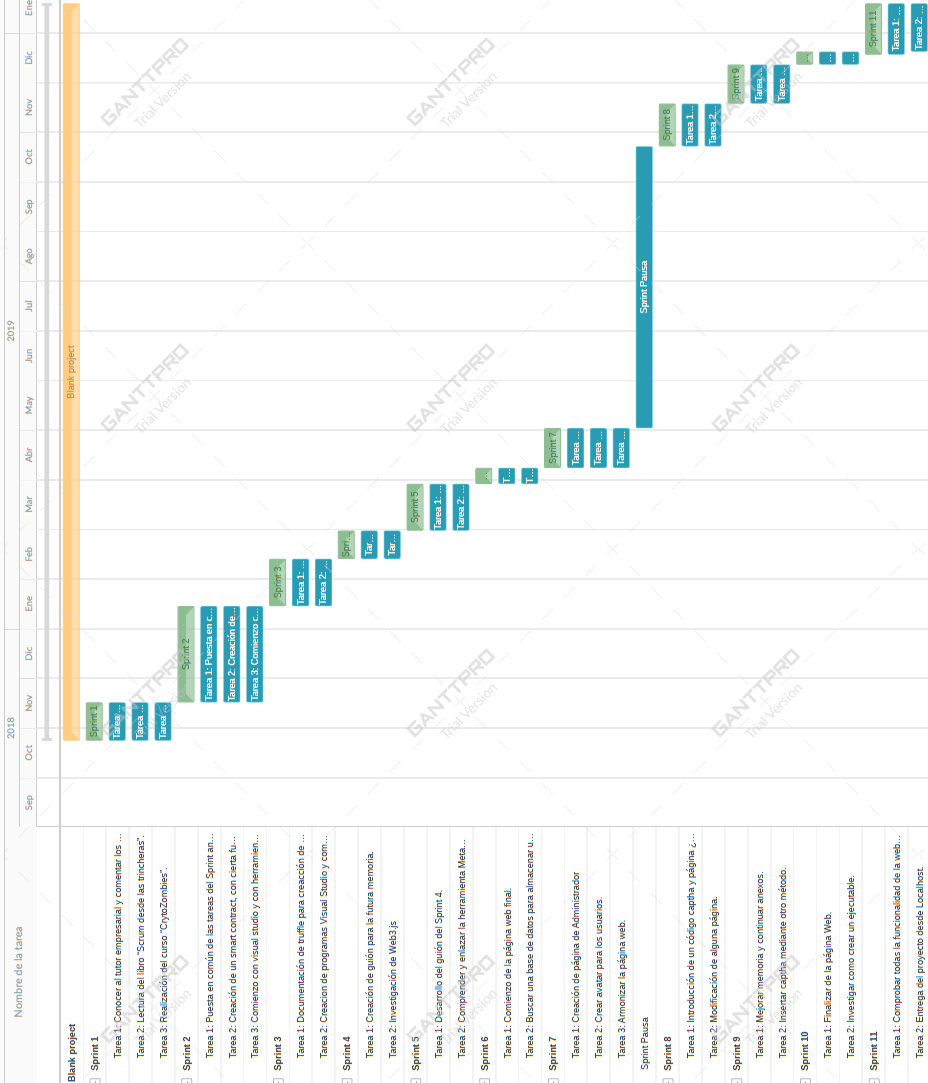
\includegraphics[width=1.00\textwidth]{dig-gantt2}
    \caption{Diagrama de Gantt}
    \label{ref:gantt}
\end{figure}

\section{Estudio de viabilidad}

En este apartado nos dispondremos a analizar los puntos de  viabilidad económica y legal, con esto podremos observar si es beneficioso o no realizar el proyecto.

\subsection{Viabilidad económica}

En el primer subapartado, expondremos costes y beneficios que tendría la realización de este proyecto en el entorno empresarial.

\subsubsection{Coste de personal}

La realización de este trabajo ha sido llevada acabo por un desarrollador junior durante 8 meses, con base en estos datos calcularemos los siguientes parámetros:

Se estima que el sueldo medio de un programador junior en España esta entre los 14.000 y los 16.000 euros brutos anuales. Para este calculo tomaremos la cifra de 14.000 euros , a este coste tendremos que añadir la parte proporcional a la seguridad social, la cual corre a cargo de la empresa, que es el 23.6\% del sueldo del empleado \cite{seguirdadSocial}. 

La estimación media para la realización del proyecto es de 13 horas semanales, compatibilizando el tiempo con la finalización del grado en ingeniería informática y realización de trabajo externo. Lo que hace un total de 416 horas empleadas en la elaboración del proyecto (8 meses * 4 semanas/mes * 13 horas/semana).


\begin{table}[h]
	\begin{center}
		\begin{tabular}{llll}
			Concepto              & Trabajador & Empresa &  \\ \hline
			Contingencias comunes & 4,7\%      & 23,6\%  &  \\ \hline
			Desempleo             & 1.55\%     & 5,5\%   &  \\ \hline
			Formación profesional & 0,1\%      & 0.6\%   &  \\ \hline 
			Garantía social       & 0          & 0.2\%   &  \\ \hline     
			TOTAL                 & 6.35\%     & 29.9\% &   \\
		\end{tabular}
	\caption{Gastos de la seguridad social}
	\label{tabla:tabla2}
	\end{center}
\end{table}

A continuación calculamos el precio hora que cobraremos, para luego calcular el salario con la seguridad social.

\begin{table}[htbp]
	\begin{center}
		\begin{tabular}{llll}
			Concepto                           & Coste (Euros)\\ \hline
			Salario anual              		   & 14.000 \\ 
			Salario mensual					   & 1166.66\\ 
			Salario a la hora                  & 7.29  \\ 
			Suelo sin seguridad social 		   & 3033.33 \\
			Sueldo con seguridad social (23.6\%)& \textbf{3749.19} \\\hline
		\end{tabular}
	\caption{Coste del empleado}
	\label{tabla:tabla3}
	\end{center}
\end{table}

Dentro de estos costes tendremos que añadir el coste del tutor.

\subsubsection{Coste informático}

Dentro de esta rama, los podremos dividir en dos clases que serán las siguientes:
 
\paragraph{Coste de hardware}

Para la realización de este proyecto, únicamente se tendrá en cuenta el coste del ordenador utilizado, el coste del ordenador ronda entre los 700 y los 900 euros.
El ordenador con el cual se ha realizado el proyecto tiene una antigüedad de 5 años y se estima un uso de vida total de 8 años y tiene un valor de 750 euros. El tiempo de empleo para este trabajo ha sido de 8 meses, por lo tanto el coste amortizado de estos meses será de 116.69 euros.

También se podrían sumar otros gastos como son luz, Internet, material de oficina pero son despreciables y por eso no se incluyen en esté calculo.

\paragraph{Coste de software}

Para la realización del proyecto, todos los programas, bibliotecas y herramientas empleadas son de software libre y gratuito. En caso de haber tenido alguna versión de pago, empleábamos la version anterior o su versión de prueba.

\subsubsection{Coste de total}

Para concluir, tendremos los siguientes costes, durante el tiempo dedicado a este proyecto, salario del empleado con la seguridad social incluida y costes informáticos.

\begin{table}[H]
	\begin{center}
		\begin{tabular}{llll}
			Concepto              & Coste (Euros)\\ \hline
			Salario total         & 3749.19  \\ \hline	
			Costes informáticos	  & 116.69    \\ \hline
			TOTAL                 & 3862.88     \\
		\end{tabular}
	\caption{Coste del empleado}
	\label{tabla:tabla4}
	\end{center}
\end{table}

El precio total del proyecto serían 3862.88 euros, esto teniendo en cuenta, que faltaría indicar de sumar el salario del tutor.

\subsubsection{Beneficio}

En cuanto a los beneficios serían inexistentes, ya que serían indirectos y se plantearía como una aplicación de uso propio para HP, con ello ayudaría en el desarrollo de la tecnología Blockchain, teniendo en cuenta en el auge de esta herramienta cada vez más usada en todos las industrias podrá ser adaptado para futuras operaciones con diferentes clientes. Asi los beneficios serían 100\% indirectos. 


\subsection{Viabilidad legal}

En este último apartado expondremos la viabilidad en el ámbito legal, hablaremos sobre las licencias software que empleamos en el desarrollo del mismo.

Se define una licencia software \cite{licencia} como un contrato mediante el cual una persona recibe de otra el derecho de uso, copia, distribución, estudio y modificación de varios de sus bienes, (normalmente de carácter intelectual), pudiéndose realizar un pago de una determinada cantidad por el uso de los mismos.

Los programas y herramientas utilizadas durante el desarrollo de este proyecto han sido de licencia abierta o de uso libre y gratuito (Solidity, HTML, PHP, Remix, Ganache \ldots). Esto es gracias a la licencia MIT ( \textit{Massachusetts Institute of Technology}) \cite{MIT}, la cual da libertad para poder usar el software libremente y con ello exime de responsabilidad a la parte creadora de las herramientas.
	
El proyecto se ha realizado en colaboración con HP SCDS, por esta razón el software resultante está bajo licencia copyright de la empresa. Asimismo, el código fuente será propiedad de HP SCDS y de la universidad de Burgos y podrá estar también bajo licencia copyright.

\apendice{Especificación de Requisitos}

\section{Introducción}
En este apartado realizaremos un estudio de requisitos y objetivos que definirán el comportamiento del proyecto actual. También hablaremos de los diferentes casos de uso y los requisitos funcionales de la herramienta en cuestión.

\section{Objetivos generales}

Los objetivos generales que se quieren alcanzar al realizar este proyecto son los siguientes:
\begin{itemize}
	\item Implementar una página web para la realización de \textit{smart contracts}, en diferentes redes y con diferentes usuarios.
	\item Investigar las posibilidades y capacidades de conexión de la red ethereum y solidity para desarrollar \textit{smart contracts}.
\end{itemize}

\section{Catalogo de requisitos}

En este apartado mencionaremos los requisitos, divididos en funcionales y no funcionales.

\subsection{Requisitos funcionales}

\paragraph{RNF-1 Crear usuarios}: crear un sistema de gestión de usuarios y permisos para, así, garantizar la seguridad de la aplicación.

\paragraph{RNF-2 Actualizar usuario}: comprobación que permita la verificación de si el usuario o la contraseña fueron modificadas y desde qué cuenta realizó los cambios.

\paragraph{RNF-3 Eliminar usuario}: revisión para saber si el usuario fue borrado desde su propia cuenta o desde la cuenta de administrador.

\paragraph{RNF-4 Comprobar captha}: verificar el botón si pasa el proceso de no soy un robot.

\paragraph{RNF-5 Conexión con metamask}: al añadir producto, comprobar que pregunta si queremos conectar con dicha aplicación.

\paragraph{RNF-6 Creación del \textit{smart contracts}}: confirmar que el contrato  fue creado desde la página web a una red Ethereum mediante metamask.

\paragraph{RNF-7 Consultar productos}: podremos consultar todos los productos, tanto el ultimo añadido o todos en forma de tabla. También se incluye la hora de la creación del contrato. 

\paragraph{RNF-8 Salir de la aplicación}: funcionalidad que permita desconectar al usuario de la página web mediante un botón.

\subsection{Requisitos no funcionales}
\paragraph{RNF-1 Usabilidad}: la aplicación será intuitiva y fácil de utilizar, así como tener una una estructura clara para qué cualquier persona pueda comprenderla sin necesidad de ninguna formación.

\paragraph{RNF-2 Eficiencia}: la aplicación funcionará de una forma fluida, sin que la interfaz gráfica quede bloqueada.

\paragraph{RNF-3 Escalabilidad}: estará siempre abierta a la incorporación de nuevas funciones o programas.

\paragraph{RNF-4 Autonomía}: deberá realizar actualizaciones para no perder información y esta siempre intente ser la más fiable posible.

\section{Especificación de requisitos}

En esta sección podremos visualizar los casos de uso de los requisitos funcionales anteriormente explicados y también detallaremos todos los casos de uso mediante tablas.

\subsection{Diagramas de casos de uso}
En las siguientes figuras podremos observar los casos de uso que corresponden a nuestra aplicación, en la cual se podrán observar dos actores (administrador y usuario). Los UML los hemos realizado en la siguiente página web \cite{uml}

\begin{figure}[h!]
    \centering
    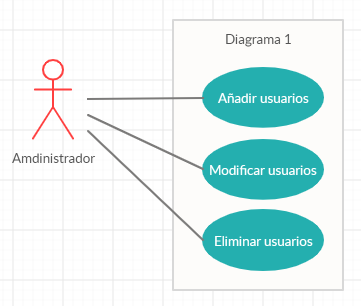
\includegraphics{CUAdmin}
    \caption{Diagrama de casos de uso del administrador}
\end{figure}

\imagen{CUUsuario}{Diagrama de casos de uso del usuario}

\subsection{Especificación de los casos de uso}

A continuación detallaremos mediante tablas los casos de uso:

\begin{table}[htbp]
	\begin{center}
		\begin{tabular}{|l|p{10cm}|}
		\hline
			\textbf{RF 1} & \textbf{Crear usuarios}                                                                                                                        			\\ \hline
			Descripción & Registro en la base de datos de nuevos usuarios.                                                                                                   \\ \hline
			Pre-condición & Un usuario deberá introducir un usuario, correo y una contraseña, con el objetivo de poder registrarse en la base de datos.\\ \hline
			Acción & Si el correo ya esta en uso, las contraseñas no coinciden o no marcamos la opción ``no soy un robot'', tendremos que repetir el proceso de registrarse. \\ \hline
			Post-condición  & Si el correo y la contraseña son correctos, nos mostrará la siguiente pantalla de la página Web.                                                     			\\ \hline
			Importancia & Alta                                                                                                                           \\ \hline
		\end{tabular}
	\caption{RF 1: Crear usuarios}
	\label{tabla:tablaB1}
	\end{center}
\end{table}

\begin{table}[htbp]
\begin{center}
\begin{tabular}{|l|p{10cm}|}
\hline
\textbf{RF 2} & \textbf{Actualizar usuario}                                                                                                                              \\ \hline
Descripción   & Dependiendo de si nos encontramos en un usuario o desde el administrador                                                                                 \\ \hline
Pre-condición   & Haber iniciado sesión previamente (desde administrador o de usuario).                                                                                    \\ \hline
Acción        & Podremos modificar el usuario y la contraseña de un usuario concreto, o, si estamos en el administrador, podremos acceder a modificar todos los usuarios. \\ \hline
Post-condición & Si todo fue correcto, los datos se modificarán en nuestra base de datos                                                                                  \\ \hline
Importancia   & Alta                                                                                                                                                     \\ \hline
\end{tabular}
\caption{RF 2: Actualizar usuarios}
	\label{tabla:tablaB2}
	\end{center}
\end{table}

\begin{table}[htbp]
\begin{center}
\begin{tabular}{|l|p{10cm}|}
\hline
\textbf{RF 3} & \textbf{Eliminar usuario}                                                                                                                       \\ \hline
Descripción   & Dependiendo de si nos encontramos en un usuario o desde el administrador, podremos ver o uno o a todos.                                         \\ \hline
Pre-condición   & Haber iniciado sesión previamente (desde administrador o de usuario).                                                                           \\ \hline
Acción        & Podremos eliminar el usuario de nuestra cuenta, ,o si estamos en el administrador, podremos acceder a eliminar los usuarios que deseemos.         \\ \hline
Post-condición & Si todo fue correcto, los datos se eliminarán en nuestra base de datos, también eliminaremos todos los productos que tiene adquiridos previamente. \\ \hline
Importancia   & Alta                                                                                                                                            \\ \hline
\end{tabular}
\caption{RF 3: Eliminar usuarios}
	\label{tabla:tablaB3}
	\end{center}
\end{table}

\begin{table}[htbp]
\begin{center}
\begin{tabular}{|l|p{10cm}|}
\hline
\textbf{RF 4} & \textbf{Comprobación captha}                                                                                                 \\ \hline
Descripción   & Cuando registramos un nuevo usuario, el ultimo apartado, una vez introducidos todos los campos, es demostrar que no se es un robot. \\ \hline
Pre-condición   & Ninguna                                                                                                                      \\ \hline
Acción        & Pulsar el botón no soy un robot, y seleccionar los campos que nos pida en cada momento.                                      \\ \hline
Post-condición & Si todo fue correcto, nos creará la nueva cuenta. \\ \hline
Importancia   & Alta                                                                                                                         \\ \hline
\end{tabular}
\caption{RF 4: Comprobar captha}
	\label{tabla:tablaB4}
	\end{center}
\end{table}

\begin{table}[htbp]
\begin{center}
\begin{tabular}{|l|p{10cm}|}
\hline
\textbf{RF 5} & \textbf{Conexión con metamask}                                                                                                                                                      \\ \hline
Descripción   & Realizar contrato desde la página web con la red Ethereum.                                                                                                                          \\ \hline
Pre-condición   & Haber iniciado sesión como usuario.                                                                                                                                                 \\ \hline
Acción        & Creación de un nuevo contrato cuando pulsamos ``Añadir Producto''. Si no tenemos Metamask conectado, nos saldrá una pantalla para iniciar sesión y crear el primer \textit{smart contracts} vacío. \\ \hline
Post-condición & Añadir todos los campos vacíos que se encuentran en la página web para la creación del \textit{smart contracts}.            \\ \hline
Importancia   & Alta                                                                                                                                                                                \\ \hline
\end{tabular}
\caption{RF 5: Conexión metamask}
	\label{tabla:tablaB5}
	\end{center}
\end{table}

\begin{table}[htbp]
\begin{center}
\begin{tabular}{|l|p{10cm}|}
\hline
\textbf{RF 6} & \textbf{Creación del \textit{smart contracts}}                                                                                                                                                            \\ \hline
Descripción   & Realizar contrato desde la página web con la red Ethereum.                                                                                                                                      \\ \hline
Pre-condición   & Haber iniciado sesión y estar en la página Añadir Producto.                                                                                                                                     \\ \hline
Acción        & Pulsaremos en ``Realizar contrato'' y nos saltará una notificación en metamask para confirmar o rechazar el contrato a realizar                                                                    \\ \hline
Pos-condición & Pulsar ``confirmar'' y tras una espera nos confirmará si se realizo correctamente pudiendo ver el contrato tanto en la red privada de Ropsten o consultando los productos añadidos de la página web. \\ \hline
Importancia   & Alta                                                                                                                                                                                            \\ \hline
\end{tabular}
\caption{RF 6: Creación del \textit{smart contracts}}
	\label{tabla:tablaB6}
	\end{center}
\end{table}

\begin{table}[htbp]
\begin{center}
\begin{tabular}{|l|p{10cm}|}
\hline
\textbf{RF 7} & \textbf{Consultar productos}                                                                                \\ \hline
Descripción   & Posibilidad de informarse de los productos que un usuario ha registrado en la red Ethereum.                 \\ \hline
Pre-condición   & Haber iniciado sesión y haber añadido un producto anteriormente (si no la página nos saldrá vacía).         \\ \hline
Acción        & Ir a la página de consulta de productos para poder observar los productos añadidos.                         \\ \hline
Post-condición & Podremos ver los productos que añadió cada usuario, solo podrán verse los productos del usuario registrado. \\ \hline
Importancia   & Alta                                                                                                        \\ \hline
\end{tabular}
\caption{RF 7: Consultar productos}
	\label{tabla:tablaB7}
	\end{center}
\end{table}

\begin{table}[h!]
\begin{center}
\begin{tabular}{|l|p{10cm}|}
\hline
\textbf{RF 8} & \textbf{Salir de la aplicación}                                \\ \hline
Descripción   & Cerrar sesión de nuestra página web.                           \\ \hline
Pre-condición   & Haber iniciado sesión.                                         \\ \hline
Acción        & Pulsar el botón de cerrar sesión, ubicado en su propio avatar. \\ \hline
Post-condición & Al cerrar sesión se desconectará de la pagina web.             \\ \hline
Importancia   & Alta                                                           \\ \hline
\end{tabular}
\caption{RF 8: Salir de la aplicación}
	\label{tabla:tablaB8}
	\end{center}
\end{table}

\apendice{Especificación de diseño}

\section{Introducción}

En este apartado de los anexos, explicaremos la forma que se resolvieron diferentes especificaciones y los casos de uso mencionados en el apartado anterior. Se intentarán analizar el porqué de las tomas de decisiones. Los diseños se dividen en:

\begin{itemize}
	\item Diseño de datos.
	\item Diseño procedimental.
	\item Diseño arquitectónico.
	\item Diseño de interfaz.
\end{itemize}

\section{Diseño de datos}

En este proyecto, los datos que manejaremos serán la creación de usuarios y los contratos que estos creen posteriormente.

Estos datos se almacenarán en una base de datos, aquellos contendrán el id de usuario y este irá relacionado con el resto de elementos de la tabla. Estos elementos les comentaremos a continuación cuando hablemos de la base de datos.



\subsection{Modelo de datos}

En la siguiente figura \ref{fig:modelo} se mostrará el modelo de datos.

\begin{figure}[h!]
    \centering
    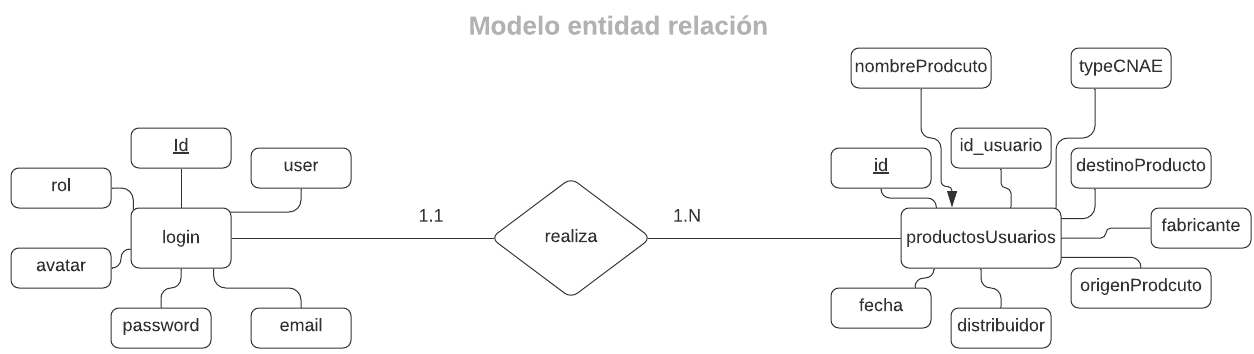
\includegraphics[width=1.00\textwidth]{modeloER}
    \caption{Modelo de datos}
    \label{fig:modelo}
\end{figure}



\subsection{XAMPP}

Utilizaremos una base de datos MySql para el almacenamiento de la información de los datos de nuestra aplicación. La base de datos está compuesta por dos tablas:

\textbf{Usuarios}: en esta tabla almacenaremos la información relacionada con la creación de nuevos usuarios registrados previamente. Esta formado por siete campos, que son los siguientes:
\begin{figure}[H]
    \centering
    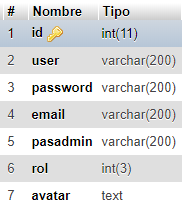
\includegraphics[width=0.60\textwidth]{loginBD}
    \caption{Tabla de usuarios}
\end{figure}
\begin{itemize}
	\item \textit{ID}: es la clave primaria (PK) y almacenará un valor único por cada usuario. Este valor es autoincremental.
	\item \textit{User}: donde se guarda el valor del usuario registrado.
	\item \textit{Password}: guardaremos la contraseña que indicó el usuario, esta a su vez se guardará de forma codificada mediante sha-1.
	\item \textit{Email}: en este campo guardaremos el correo del usuario, el cual será un campo único y, en caso de introducir el mismo, no nos dejará guardarlo de nuevo
	\item \textit{Pasaadmin}: campo diseñado para guardar la contraseña en caso de ser los administradores de la página. Este campo actualmente no está en uso ya que descartamos la opción de poder crear administradores nuevos.  	
	\item \textit{Rol}: tendrá dos posibles valores, dependiendo de si somos los administradores o, por el contrario, somos los usuarios de la página. Los valores sera 1 o 2 respectivamente.
	\item \textit{Avatar}: en el último campo tendremos la foto predeterminada del usuario en caso de que haya seleccionado foto a la hora de registrarse, si no está, será una foto neutra.
\end{itemize}

\textbf{Productos de los usuarios}: en esta nueva tabla se almacenarán todos los productos que el usuario, previamente registrado, ha realizado en la red de Ethereum. Hay un total de diez campos y son los siguientes:
 
\begin{figure}[h]
    \centering
    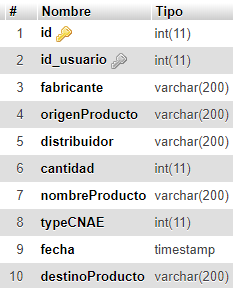
\includegraphics[width=0.80\textwidth]{productoBD}
    \caption{Tabla de productos}
\end{figure}

\begin{itemize}
	\item \textit{Id}: es la clave primaria de la tabla (PK), el valor es auto incremental haciendo que cada producto posea un identificador único.
	\item \textit{Id usuario}: es la clave foránea, la cual se relaciona con la clave primaria de la tabla anterior (usuarios). Gracias a esto tendremos siempre relacionada la tabla usuarios con la de productos, gracias al Id del usuario.
	\item \textit{Fabricante}: indica a quién estamos pidiendo el producto cada vez. Se trata de un campo de caracteres.
	\item \textit{OrigenProducto}: nos referimos de dónde saldrá el paquete en su origen, es un campo de caracteres.
	\item \textit{Distribuidor}: indicaremos quién es el encargado del reparto en cada producto registrado, este campo es de caracteres. 
	\item \textit{Cantidad}: hará referencia al número que queremos adquirir para el pedido de ese producto, este campo es numérico. 
	\item \textit{NombreProducto}: nos referimos al nombre concreto del producto que deseamos adquirir, este campo será de caracteres.
	\item \textit{TypeCNAE}: indicaremos mediante un valor numérico la Clasificación Nacional de Actividades Económicas (CNAE).
	\item \textit{Fecha}: recogeremos la hora en la que se realizó el contrato en nuestra red, este tiempo puede variar unos segundos  la red Ethereum.
	\item \textit{DestinoProdcuto}: es lo mismo que el origenProdcuto, pero esta vez tendremos que indicar el punto final del paquete, es un campo de caracteres.	
\end{itemize}

\section{Diseño procedimental}

En este punto, explicaremos el comportamiento de la aplicación y veremos los procedimientos o funcionalidades que existen en el proyecto. En bases generales esto intenta ser lo más intuitivo y eficaz para que lo pueda usar todo tipo de usuarios.

Contamos con una base de datos ya creada, la cual contará con las dos tablas previamente explicadas, dichas tablas no se podrán modificar.

Tendremos dos tipos de entrada en la página web, podrán ser mediante administrador, o bien, mediante usuario.

La siguiente imagen muestra el diagrama de flujo \ref{fig:diagrama} el inicio de sesión de la página web:

\begin{figure}[H]
    \centering
    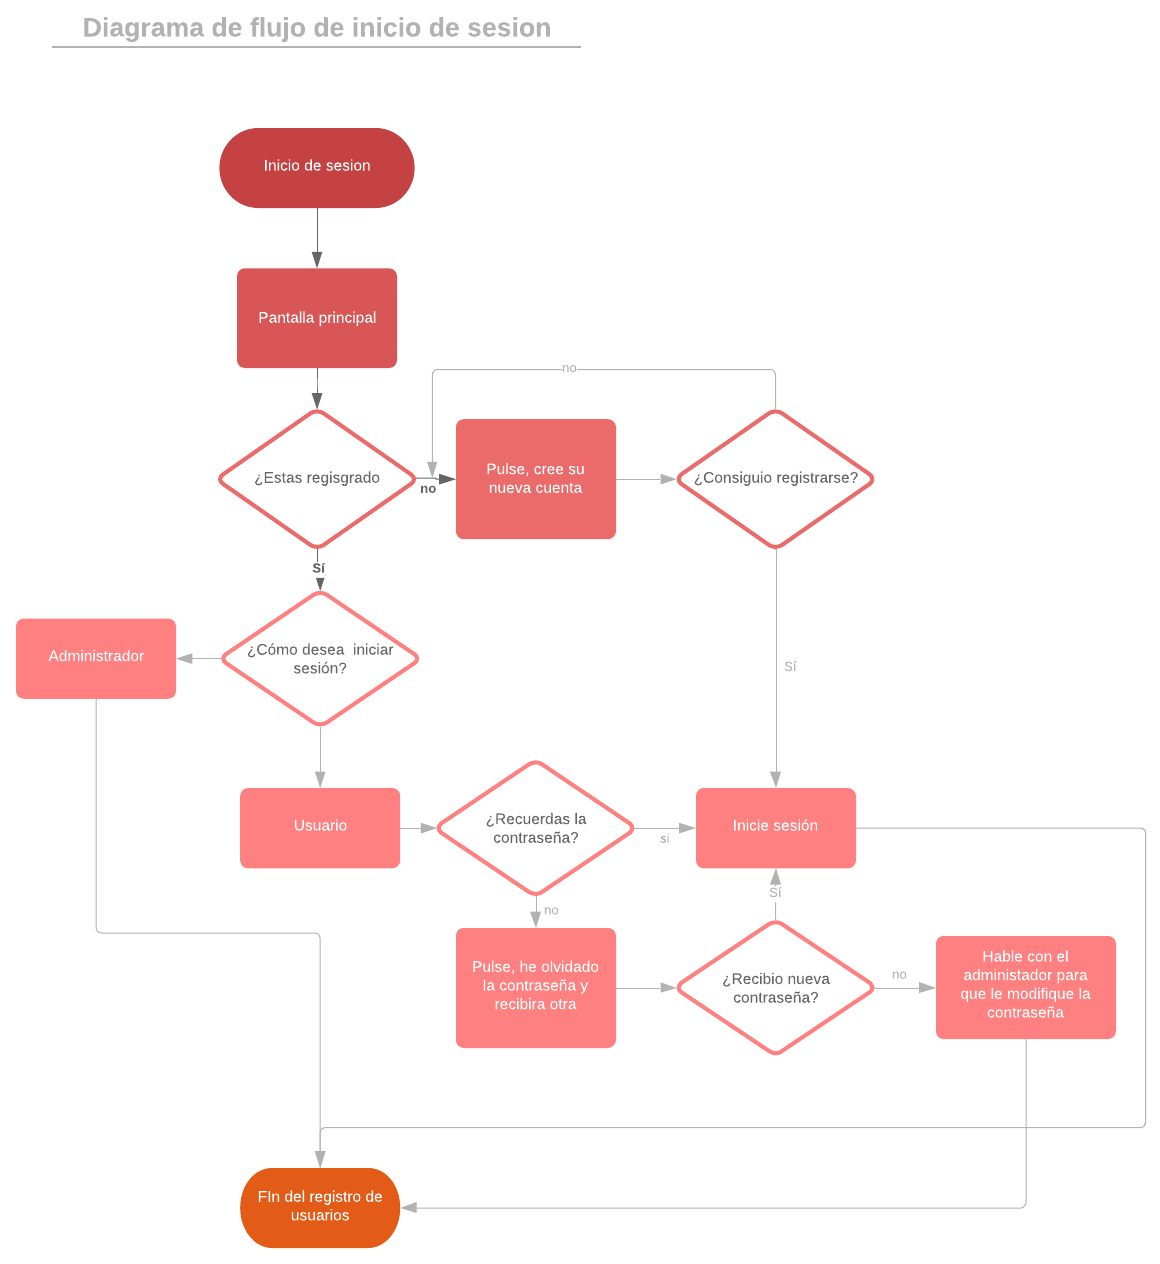
\includegraphics[width=0.60\textwidth]{diagramaFlujo}
    \caption{Diagrama de flujo de inicio de sesión}
    \label{fig:diagrama}
\end{figure}

En la siguiente imagen mostraremos el funcionamiento de la página una vez, hemos registrado sesión, dependiendo de si estamos en modo administrador o modo usuario \ref{fig:funcionamiento}.

\begin{figure}[H]
    \centering
    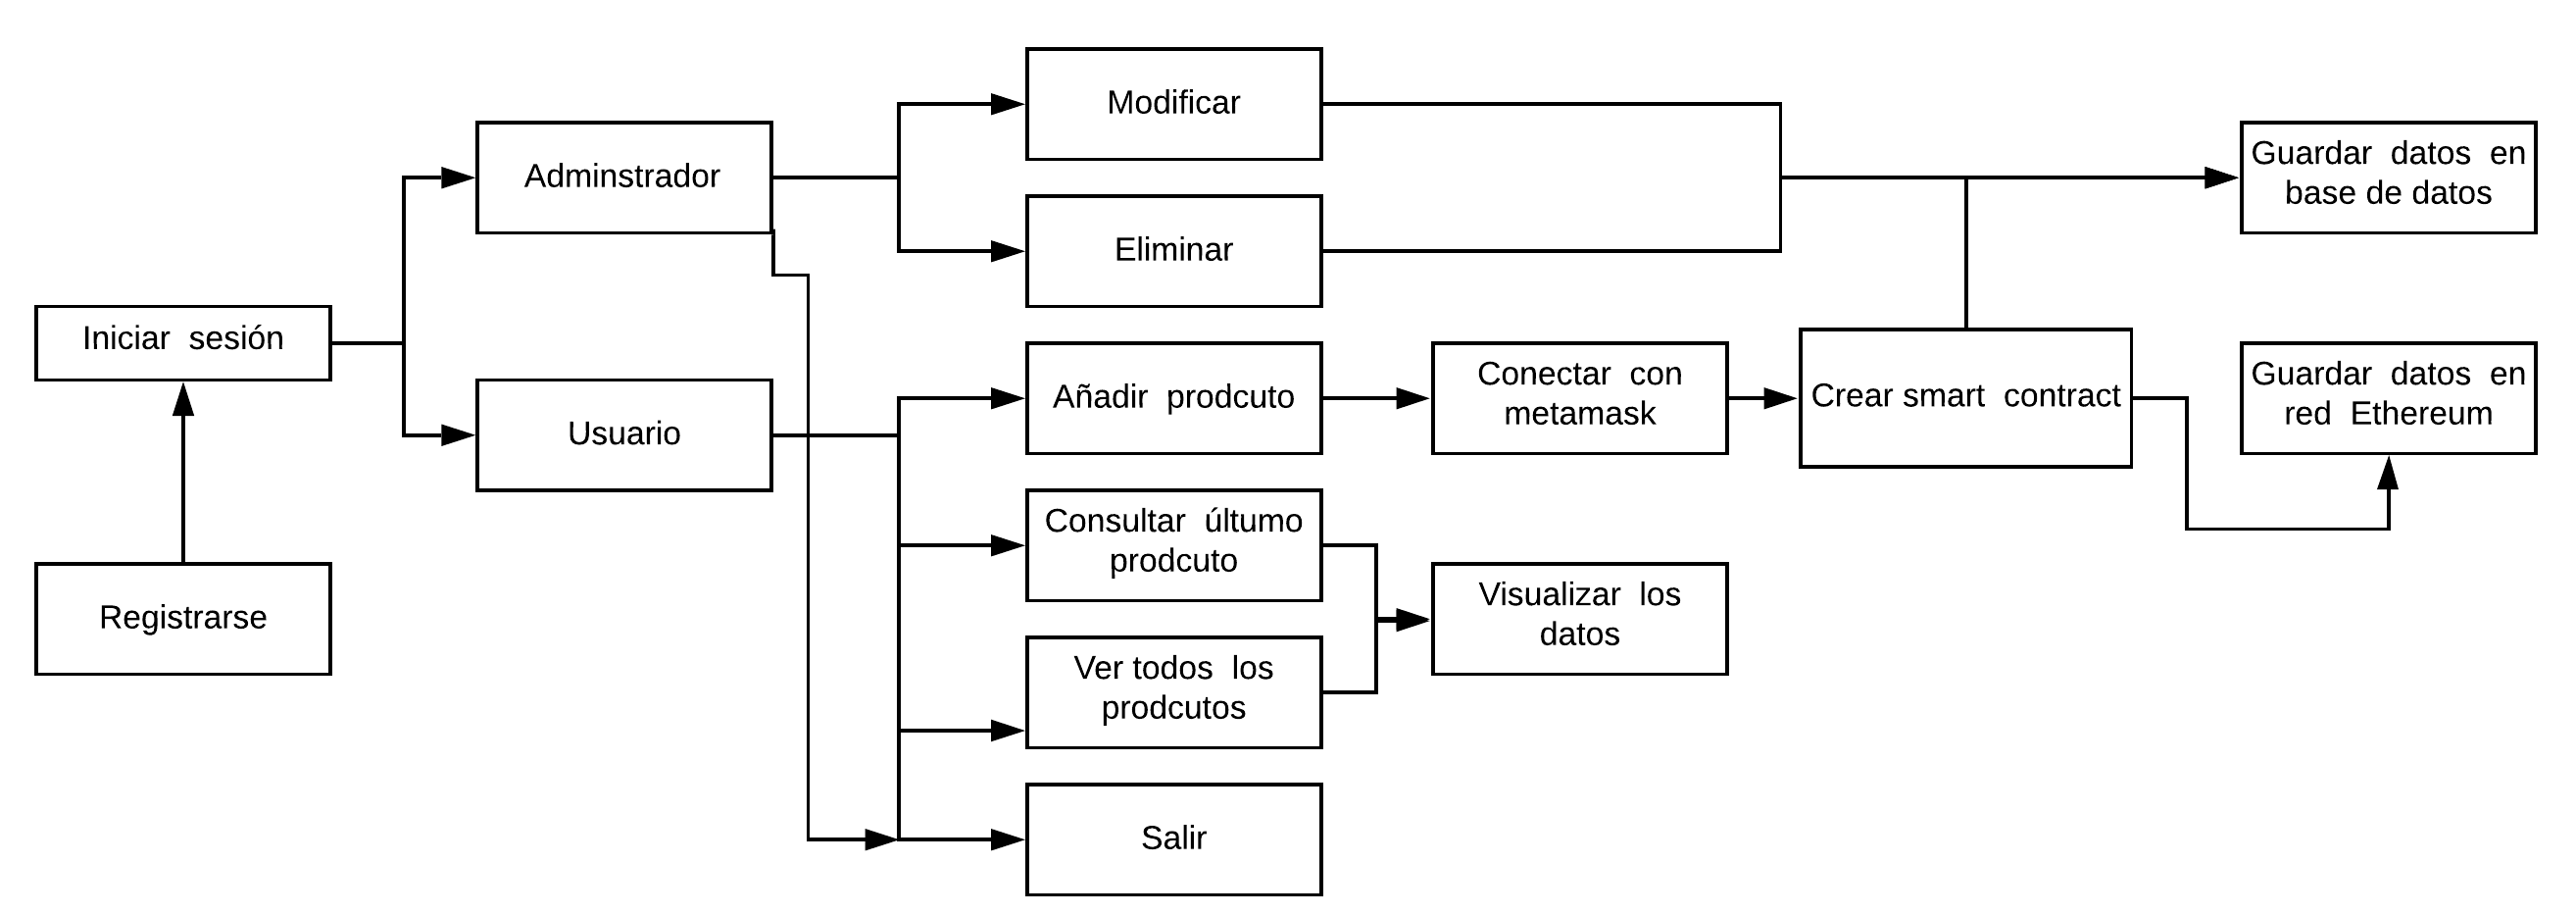
\includegraphics[width=1.00\textwidth]{funcionamientoPag}
    \caption{Tabla de productos}
    \label{fig:funcionamiento}
\end{figure}

A continuación, explicaremos las funciones que coinciden del usuario y del administrador:

\begin{enumerate}
	\item \textbf{Modificar}:
	\begin{itemize}
		\item \textit{Usuario}: podrá cambiar tanto el nombre y la contraseña de su propio usuario.
		\item \textit{Administrador}: tendrá acceso a cambiar el nombre y contraseña de todos los usuarios registrados en la base de datos, también podrá acceder a ver el id de los usuarios.
\end{itemize}			
\item \textbf{Eliminar}:
	\begin{itemize}
		\item \textit{Usuario}: dispondrá de una opción para eliminar su propia cuenta y todos los productos asociados a él.
		\item \textit{Administrador}: tendrá acceso a visualizar todos los usuarios registrados en la base de datos y podrá eliminar los que desee, esto también elimina todos los productos asociados previamente.
	\end{itemize}			
\item \textbf{Salir}:
	\begin{itemize}
		\item \textit{Usuario y administrador}: podremos salir una vez estemos registrado en la página web.
	\end{itemize}			
\end{enumerate}

\section{Diseño arquitectónico}

Para la creación de la interfaz de usuario, los requisitos que deseábamos cumplir eran facilidad y sencillez a la hora de usar la página web. La interfaz es clara y  limpia, con esto se consigue facilitar la interacción con el usuario. Esto se logra gracias a las páginas de estilo (css) y utilizando los \textit{bootstrap} que resulta en que la página quede con buen aspecto visual.
%\begin{figure}[H]
%	\begin{minipage}[b]{1.00\linewidth}
%		\centering
%		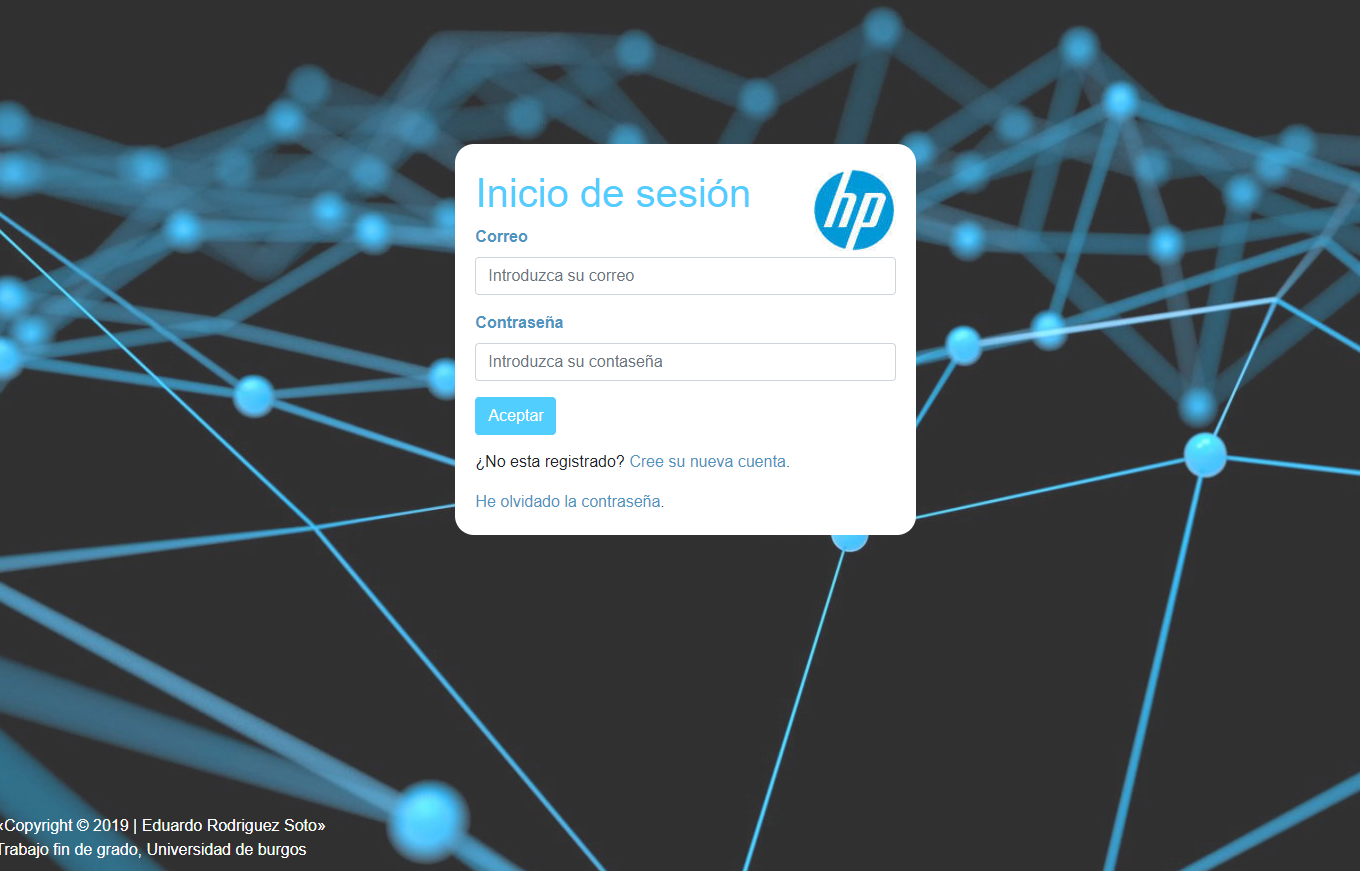
\includegraphics[width=1.00\textwidth]{incioPag}
%		\caption{Inicio de sesión}
%		\label{fig:inicio}
%	\end{minipage}
%	\hspace{0.3cm}
%	\begin{minipage}[b]{1.0\linewidth}
%		\centering
%		
\includegraphics[width=1.00\textwidth]{index}
%		\caption{Usuario registrado}
%		\label{fig:registrado}
%	\end{minipage}
%\end{figure}

En el apéndice \ref{ref:front} realizaremos la explicacion del \textit{front-end} de la aplicación final, para que el usuario pueda tener una guía explicativa. 

Con el objetivo de ayudar al usuario, hemos incorporado mensajes de aviso, tanto si son de error \ref{fig:error}, si son informativos \ref{fig:correcto} o son preguntas de confirmación \ref{fig:confirmar}.

\begin{figure}[H]
	\begin{minipage}[b]{0.5\linewidth}
		\centering
		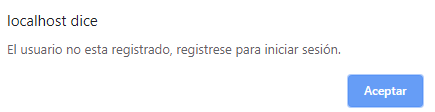
\includegraphics[width=1.00\textwidth]{error}
		\caption{Mensaje correo no registrado en la base de datos}
		\label{fig:error}
	\end{minipage}
	\hspace{0.3cm}
	\begin{minipage}[b]{0.5\linewidth}
		\centering
		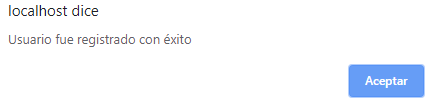
\includegraphics[width=1.00\textwidth]{correcto}
		\caption{Mensaje de usuario creado con éxito}
		\label{fig:correcto}
	\end{minipage}
	\\
	\begin{minipage}[b]{0.5\linewidth}
		\centering
		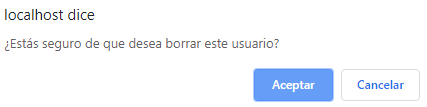
\includegraphics[width=1.00\textwidth]{confirmar}
		\caption{Mensaje de confirmar proceso}
		\label{fig:confirmar}
	\end{minipage}
\end{figure}






\apendice{Documentación técnica de programación}

\section{Introducción}

La documentación técnica de programación describirá la estructura de los programas empleados en el proyecto, el entorno de desarrollo, la instalación y ejecución de los programas.

\section{Estructura de directorios}

Dentro de GitLab tendremos programas y códigos que nos resultaran ajenos para el correcto funcionamiento, estos programas son pruebas realizadas anteriormente (tutoriales, código de pruebas \ldots).

Para el desarrollo del proyecto \footnote{Repositorio GitLab: \url{https://gitlab.com/HP-SCDS/Observatorio/2018-2019/ubu-bc4distribution/tree/paginaWeb}} \footnote{Repositorio GitHub: \url{https://github.com/ers0026/ProyectoFinal}}, se utiliza los siguientes ramas:

\begin{itemize}
	\item \textit{Proyecto}: en la raíz \textbackslash xampp\textbackslash htdocs\textbackslash proyectoFinal tendremos todo el contenido del código de nuestro proyecto, archivos: PHP, CSS, Bootstrap \ldots y también el enlace de conexión con metamask.
	\item \textit{Documentación}: se encontrará en la carpeta Latex y contará con la documentación (memoria y anexos) para la compresión del funcionamiento de la aplicación, también cuenta con un guion de la instalación de truffle, el cual no hace falta para el funcionamiento pero creemos que un buena herrmienta para el funcionamiento del proyecto). También se dispondrán los pdf en la rama principal para su fácil acceso.
\end{itemize}

\section{Manual del programador}

En esta sección hablaremos de la instalación de los programas necesarios para el funcionamiento de la página web y su conexión con la red Ethereum.

\begin{itemize}
	\item \textbf{Metamask\label{ref:install}} 
	\begin{itemize}
		\item Primeramente realizaremos la instalación en el navegador que deseemos desde la página\footnote{\url{https://metamask.io/}} (en nuestro caso lo hemos realizado desde Google Chrome).
		\item Ahora nos redireccionará y nos aparecerá un botón ``Añadir a Chrome''. 
		\item A continuación nos saldrá una pantalla emergente: ``Añadir extensión''. 
		\item Esto instalará en la barra de extensiones el símbolo de metamask, un zorro. 
	\end{itemize}

Después de estos pasos, tendremos una serie de pasos a realizar para importar la cuenta:
	
	\begin{itemize}
		\item Primera imagen indica el comienzo de metamask \ref{fig:Metamask1}, pulsaremos ``\textit{Get Started}'' para continuar.
		\item Seguidamente tendremos dos caminos posibles \ref{fig:Metamask2}:
			\begin{enumerate}
				\item Continuar con una cuenta ya existente.
				\item Crear una nueva cuenta.
			\end{enumerate}
		En este caso iremos por el camino de ``\textit{Importar Wallet}'' ya que las operaciones las realizaremos desde la misma cuenta, si deseáramos cambiar de cuenta tendríamos que realizar cambios en el código.	
		\item A continuación, nos pedirá los permisos para analizar los movimientos que realizamos, pulsaremos ``\textit{I agree}''\ref{fig:Metamask3}
		\item Esta es la pantalla más importante, ya que tendremos que tener la cadena de palabras \textit{nmonic} que nos dieron al crear la cuenta por primera vez y al iniciar en otro ordenador tendremos que introducir nuevamente una contraseña para entrar futuras veces (pondremos la misma contraseña que tenemos en otros navegadores o equipos) para así tener acceso siempre a nuestro metamask y aceptaremos los terminos de uso. Una vez todo este realizado pulsaremos ``importar'' \ref{fig:Metamask4}
		\item Nos mostrará un mensaje de registro completado con exito \ref{fig:Metamask5} y tendremos que clic en ``All done''
	\end{itemize}
\begin{figure}[H]
	\begin{minipage}[b]{0.5\linewidth}
		\centering
		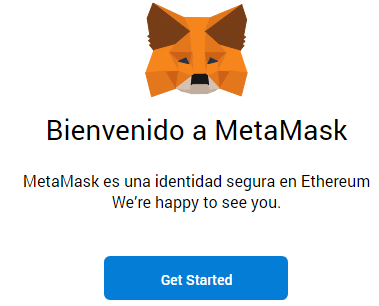
\includegraphics[width=\linewidth]{Metamask1}
		\caption{Confirmar el contrato}
		\label{fig:Metamask1}
	\end{minipage}
\hspace{0.5cm}
	\begin{minipage}[b]{0.5\linewidth}
		\centering
		\includegraphics[width=\linewidth]{Metamask2}
		\caption{Conexión pendiente}
		\label{fig:Metamask2}
	\end{minipage}
	\begin{minipage}[b]{0.5\linewidth}
		\centering
		\includegraphics[width=\linewidth]{Metamask3}
		\caption{Confirmar el contrato}
		\label{fig:Metamask3}
	\end{minipage}
\hspace{0.5cm}
	\begin{minipage}[b]{0.5\linewidth}
		\centering
		\includegraphics[width=\linewidth]{Metamask4}
		\caption{Conexión pendiente}
		\label{fig:Metamask4}
	\end{minipage}
	\begin{minipage}[b]{0.8\linewidth}
		\centering
		\includegraphics[width=\linewidth]{Metamask5}
		\caption{Conexión confirmada}
		\label{fig:Metamask5}
	\end{minipage}
\end{figure}

		
	\item \textbf{XAMPP}
	
Para descargar el programa XAMPP, tendremos que seguir los siguientes pasos:	
	\begin{enumerate}
		\item Iremos a la página\footnote{\url{https://www.apachefriends.org/index.html}}.
		\item Elegiremos la versión en la que ejecutaremos XAMPP (Windows, Linux o iOS.
		\item Una vez descargado, buscaremos el archivo ``xampp-win32-7.2.4-0-VC15-installer'' y ejecutaremos el archivo.
		\item Cuando se abra la primera pantalla, haremos clic en \textit{Yes}.
		\item A continuación seleccionaremos las funciones XAMPP que deseamos instalar, en nuestro caso seleccionamos todas ellas, será la forma predeterminada y pulsaremos ``\textit{Next}''.
		\item Seleccionaremos la ubicación donde deseemos instalar el programa. Una vez ubicado pulsaremos ``\textit{Next}''.
		\item En la penúltima pantalla desmarcaremos la opción de ``textit{Learn more about Bitnami for XAMPP}'' ``Aprender más sobre Bitnami'' y clicamos ``\textit{Next}''.
		\item Con esto empezará a instalar XAMPP en la carpeta seleccionada. Pulsaremos \textit{Finish}, esto cerrará la ventana y abrirá el panel de control de XAMPP y aquí accedemos a los servidores. Antes de ello, tendremos que seleccionar el idioma que deseemos. 
	\end{enumerate}	
	\item \textbf{Visual Stuido Code}
	\begin{enumerate}
		\item Nos dirigiremos a la página\footnote{\url{https://code.visualstudio.com/}} y seleccionaremos para qué sistema deseamos el programa: Windows, Linux, macOS.
		\item Una vez descargado, se abrirá un asistente de instalación y tendremos que aceptar el acuerdo de licencia y pulsaremos ``siguiente''.
		\item Elegiremos la carpeta donde instalará el programa.
		\item La siguiente pantalla nos preguntara sobre las tareas adicionales que queremos realizar, una vez seleccionadas pulsaremos siguiente.
		 \item La penúltima pantalla, clicaremos sobre ``instalar''. Una vez finalizado nos preguntará si deseamos ejecutarle por primera vez y pulsaremos ``finalizar''.
		 \item  Ahora, cada vez que queremos iniciar el programa, sólo tendremos que pulsar sobre el icono creado de Visual Studio Code para iniciar el programa. 
	\end{enumerate}	
\end{itemize}

\section{Compilación, instalación y ejecución del proyecto}\label{intalacionE}

\subsection{Descarga del proyecto}
En este apartado explicáramos los pasos a realizar para poder tener la aplicación web en nuestro ordenador y poder coger la base de datos y poder operar con ella directamente. 

Para la obtención del código y los recursos del proyecto, tendremos que dirigirnos al repositorio de GitLab desde el siguiente enlace\footnote{Repositorio GitLab: \url{https://gitlab.com/HP-SCDS/Observatorio/2018-2019/ubu-bc4distribution/tree/paginaWeb}} \footnote{Repositorio GitHub: \url{https://github.com/ers0026/ProyectoFinal}}.

Tendremos que descargar la carpeta XAMPP, primeramente habrá que descomprimirlo y guardarlo directamente en (C:), seguidamente dentro de la carpeta XAMPP encontraremos diferentes carpetas y documentos:

\begin{enumerate}
	\item En dicha carpeta buscaremos el archivo \textbf{xampp\_start.exe} \ref{fig:figura11}, clicaremos sobre ese ejecutable, a continuación daremos los permisos pertinentes para poder ejecutar el archivo.
	\item Con esto se activaran los módulos de Apache y MySQL. Para cerciorarnos que están activados tendremos que ejecutar \textbf{xampp\_control.exe} \ref{fig:figura11} y ejecutar desde los comandos \textit{START} de Apache y MySQL que tenemos en fosforito en la imagen \ref{fig:figura12}.
\end{enumerate}

\begin{figure}[h!]
	\centering
	\begin{minipage}[b]{0.8\linewidth}
		\centering
		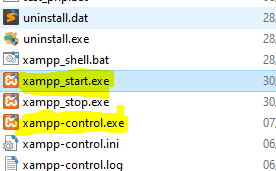
\includegraphics[width=\linewidth]{XAMPPautomatico}
		\caption{Ejecución de XAMPP automáticamente}
		\label{fig:figura11}
	\end{minipage}
	\begin{minipage}[b]{0.8\linewidth}
		\centering
		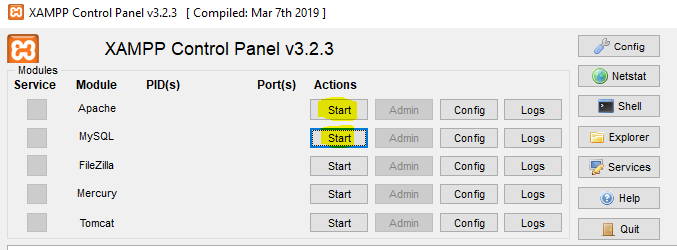
\includegraphics[width=\linewidth]{XAMPPmanual}
		\caption{Ejecución de XAMPP manualmente}
		\label{fig:figura12}
	\end{minipage}
\end{figure}


Así ya tendremos nuestra base de datos local activada y tendremos que dirigirnos a nuestro navegador para poner en nuestro navegador: localhost/proyectoFinal (proyectoFinal, ya que es así como se llama la carpeta donde tenemos el código de la página web).

Una vez estemos visualizando la página web en el modo local, nos servirá de ayuda el punto Interfaz gráfica \textit{Front-End} \ref{ref:front}

Una vez descargado el archivo y tengamos acceso a la página web tendremos que instalar Metamask \ref{ref:install}

Metamask: tendremos que estar registrados previamente o, si no, al añadir producto nos saldrá una pantalla para introducir la contraseña\footnote{La contraseña la tendremos en un archivo en el GitLab, el archivo se llama nemonic metamask.txt} y a continuación nos desplegará el primer contrato. Para comenzar a funcionar tendremos que  seleccionar la Red privada Ropsten.

\apendice{Documentación de usuario}

\section{Introducción}

En el último apéndice, indicaremos lo que necesitarán los usuarios de nuestra aplicación.

\section{Requisitos de usuarios}
 Enumeraremos los requisitos que se tienen que tener para poder usar la aplicación:
\begin{itemize}
 \item Si fuera la primera vez que vamos trabajar con está página, tendremos que descargarnos la base de datos y el código de la página del repositorio GitLab.
 \item La extensión de metamask, en el navegador en el que despleguemos la pagina web.
 \item Conexión a Internet, ya que la página web el código cuenta con iconos que cogemos directamente de internet.
\end{itemize}
 
\section{Instalación}

Únicamente tendremos que descargar la extensión de metamask y la base de datos y código del repositorio GitLab \ref{intalacionE}.

\section{Manual del usuario}

Este manual va a constar la parte del administrador y usuario, el administrador podrá controlar a los usuarios y los usuarios podrán crear añadir nuevos productos y visualizar los productos que el mismo realizo. 

\subsection{Interfaz gráfica \textit{Front-End}\label{ref:front}}

En este apartado mostraremos el aspecto final de nuestra aplicación.

En este apartado explicaremos las diferentes pantallas de nuestra página web, y como consigue realizar la conexión con el método de pago mediante Metamask, y comprobar mediante la red Ethereum que el contrato se creó correctamente.

\paragraph{Inicio de sesión}\ref{fig:inicio}: la primera pantalla, nos resultará familiar de otras paginas web, hemos intentado que la página sea concisa, fácil e intuitiva. 

\begin{figure}[H]
    \centering
    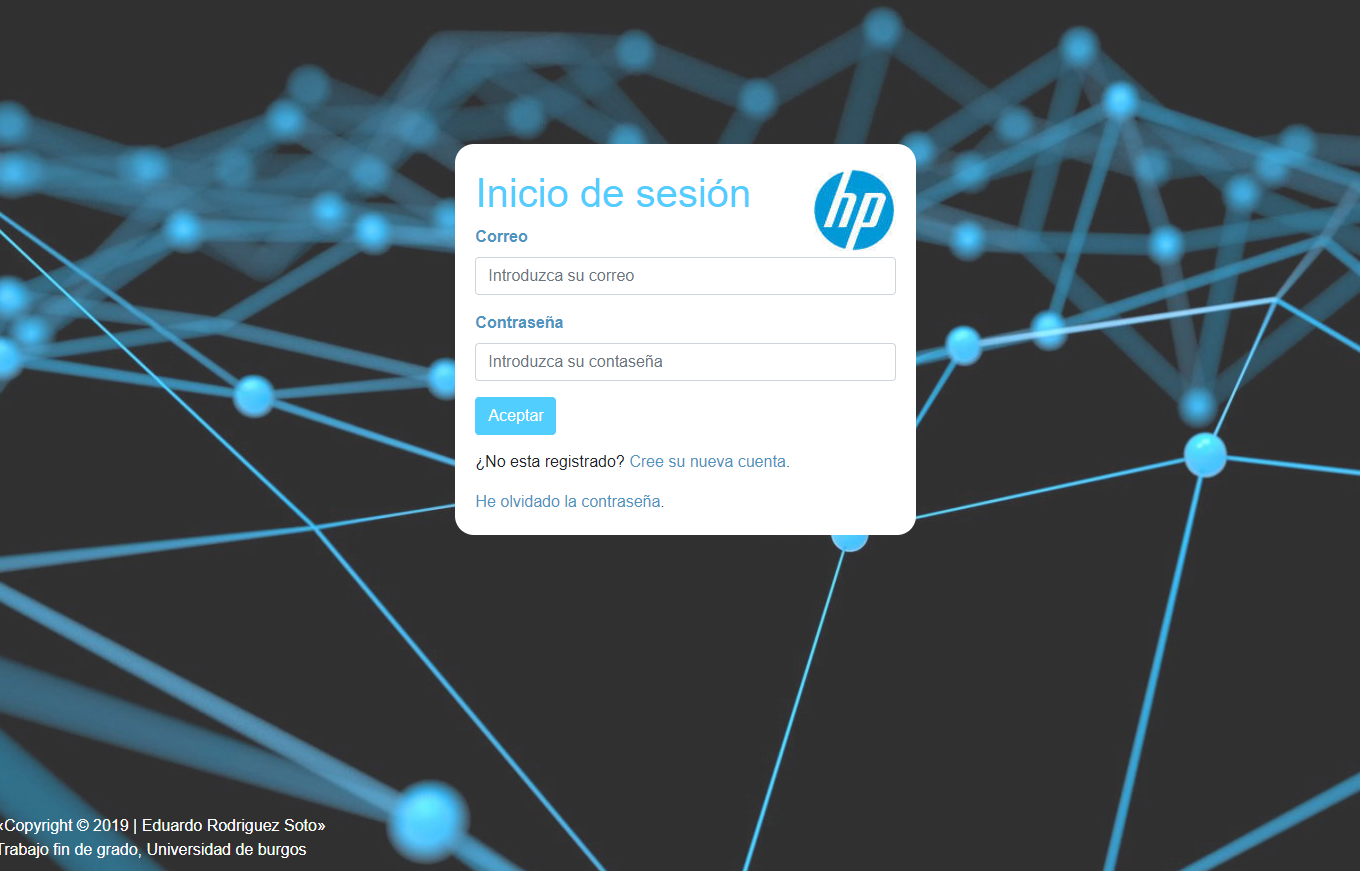
\includegraphics[width=\textwidth]{incioPag}
    \caption{Inicio de sesión}
    \label{fig:inicio}
\end{figure}

Tendremos que introducir el correo y la contraseña que previamente hayamos indicados a la hora de registrarnos y que tendremos en la misma página en un enlace ``¿No esta registrado? Cree su nueva cuenta''. En cualquier caso, si introducimos mal los datos, nos saltará mensaje de error y nos pedirá volver a iniciar sesión, teniendo la opción de poder enviarnos un correo de recordatorio de la contraseña al correo con el que nos registramos.

\paragraph{Crear nueva cuenta} \ref{fig:registro}: al igual que muchas páginas web, hemos creado la pantalla de registro (a esta página llegaremos desde la pantalla de inicio de sesión en la cual tendremos un apartado, ``¿No esta registrado? Cree su nueva cuenta''). Esta pantalla se compondrá de los campos: nombre, avatar, correo, contraseña, repetir contraseña y comprobación de que no eres un robot.

Todos los campos serán obligatorios, excepto el avatar, que en caso de no seleccionar ninguno, se le asignará el que tenemos por defecto.

\begin{figure}[h!]
    \centering
    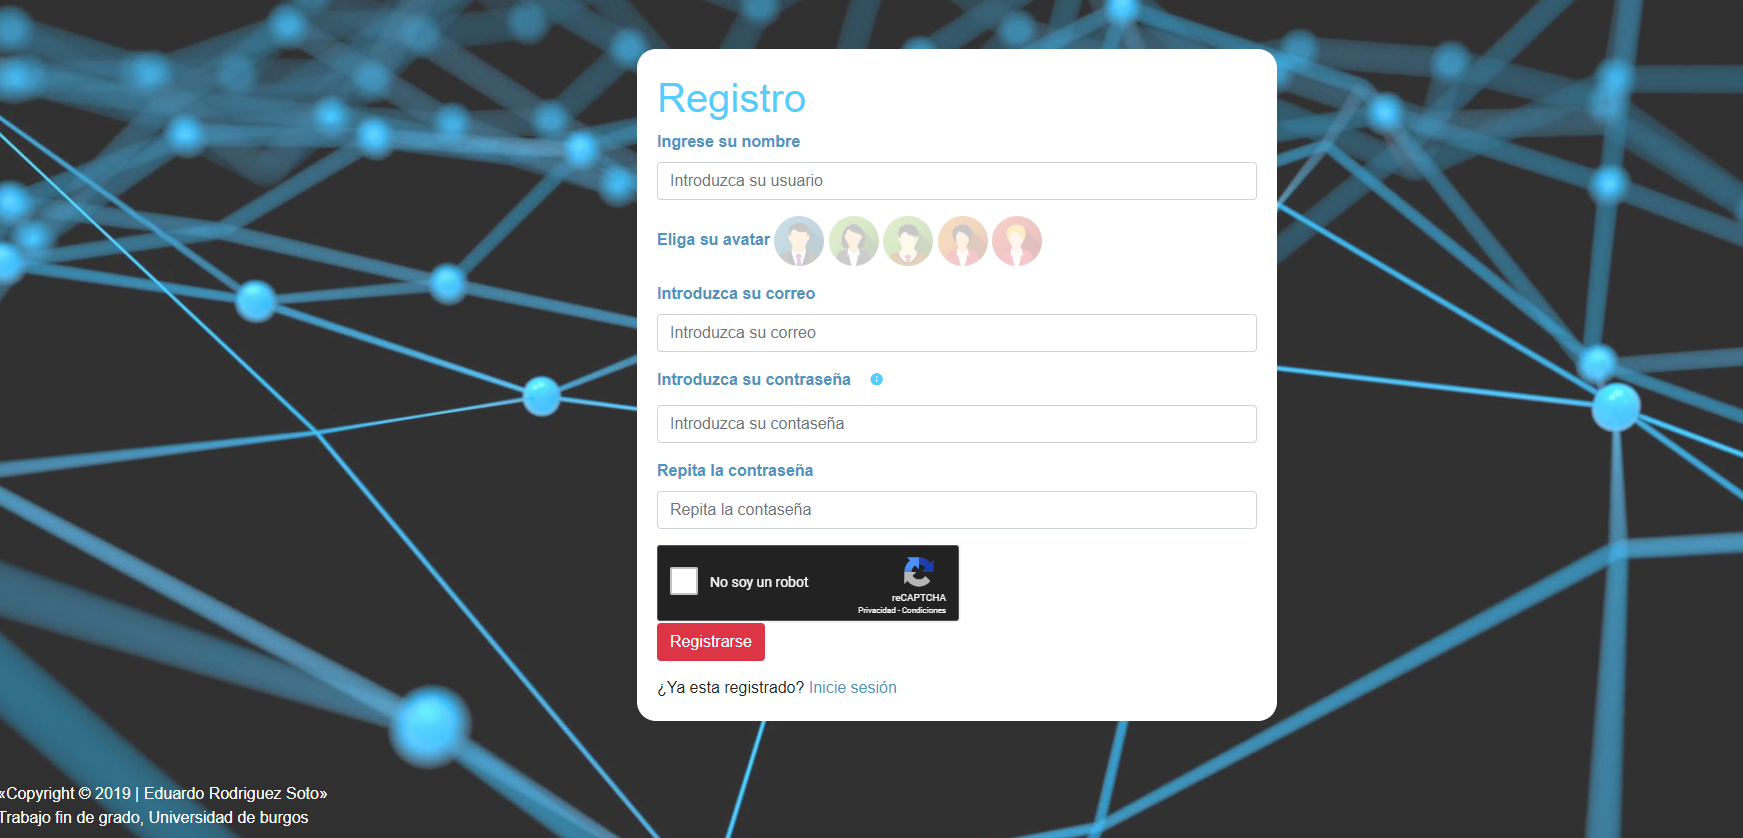
\includegraphics[width=\textwidth]{registro}
    \caption{Registrar nueva cuenta}
    \label{fig:registro}
\end{figure}

La contraseña tendrá que tener un formato típico (incluyendo mayúscula, minúscula y un número, y tendrá que ser compuesta de una cadena entre 8 y 12 elementos). En el caso de no introducir bien ambas contraseñas nos mostrará un error y nos llevará a la misma pantalla nuevamente, para volver a realizar el registro del usuario. En el caso de meter un correo ya existente a la hora de registrarse nos informará que ese correo ya está registrado. 

\paragraph{Olvido su contraseña} \ref{fig:olvido} suponemos que todo el mundo comete errores, y uno de los mas comunes es poder olvidar la contraseña, por ello hemos creado desde la pantalla de inicio de sesión, la opción de ``He olvidado la contraseña'', pinchando en en el enlace nos redirige a una página, la cual nos pedirá el correo del usuario, para así poder enviar un mensaje a su correo. Este nos dará una contraseña temporal para que el usuario pueda entrar en la cuenta y después modificar la contraseña, dependiendo si él quiere o no, en caso que el correo no esté en la base de datos, nos dará un mensaje de error de que ese usuario no está registrado\footnote{Esta página al trabajar en modo LocalHost, no estará habilitada, pero esta programada para funcionar cuando dispongamos de un dominio}.  s

\begin{figure}[H]
    \centering
    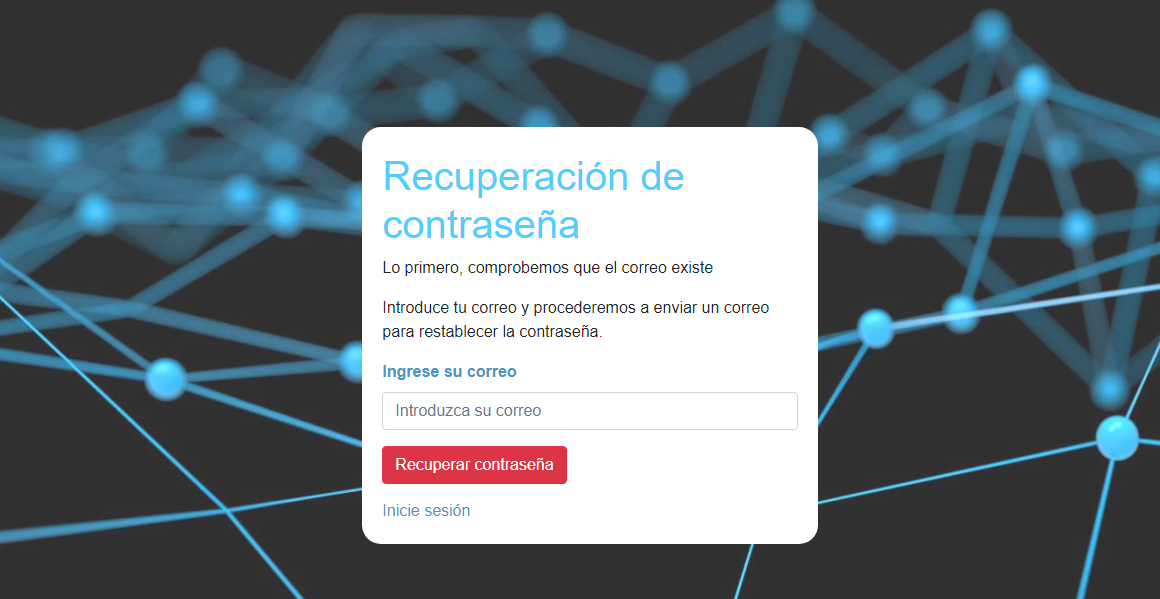
\includegraphics[width=\textwidth]{recuperarCnt}
    \caption{Recuperar contraseña}
    \label{fig:olvido}
\end{figure}

\paragraph{Página del administrador} \ref{fig:admin}: una vez reconocemos todos los enlaces de la pantalla de inicio, es hora de poder entrar en la sesión. Tendremos dos maneras de entrar: mediante el registro en la aplicación o por el uso de administrador, el cual será (admin/admin). Tendremos una pantalla como la siguiente: 

 \begin{figure}[H]
    \centering
    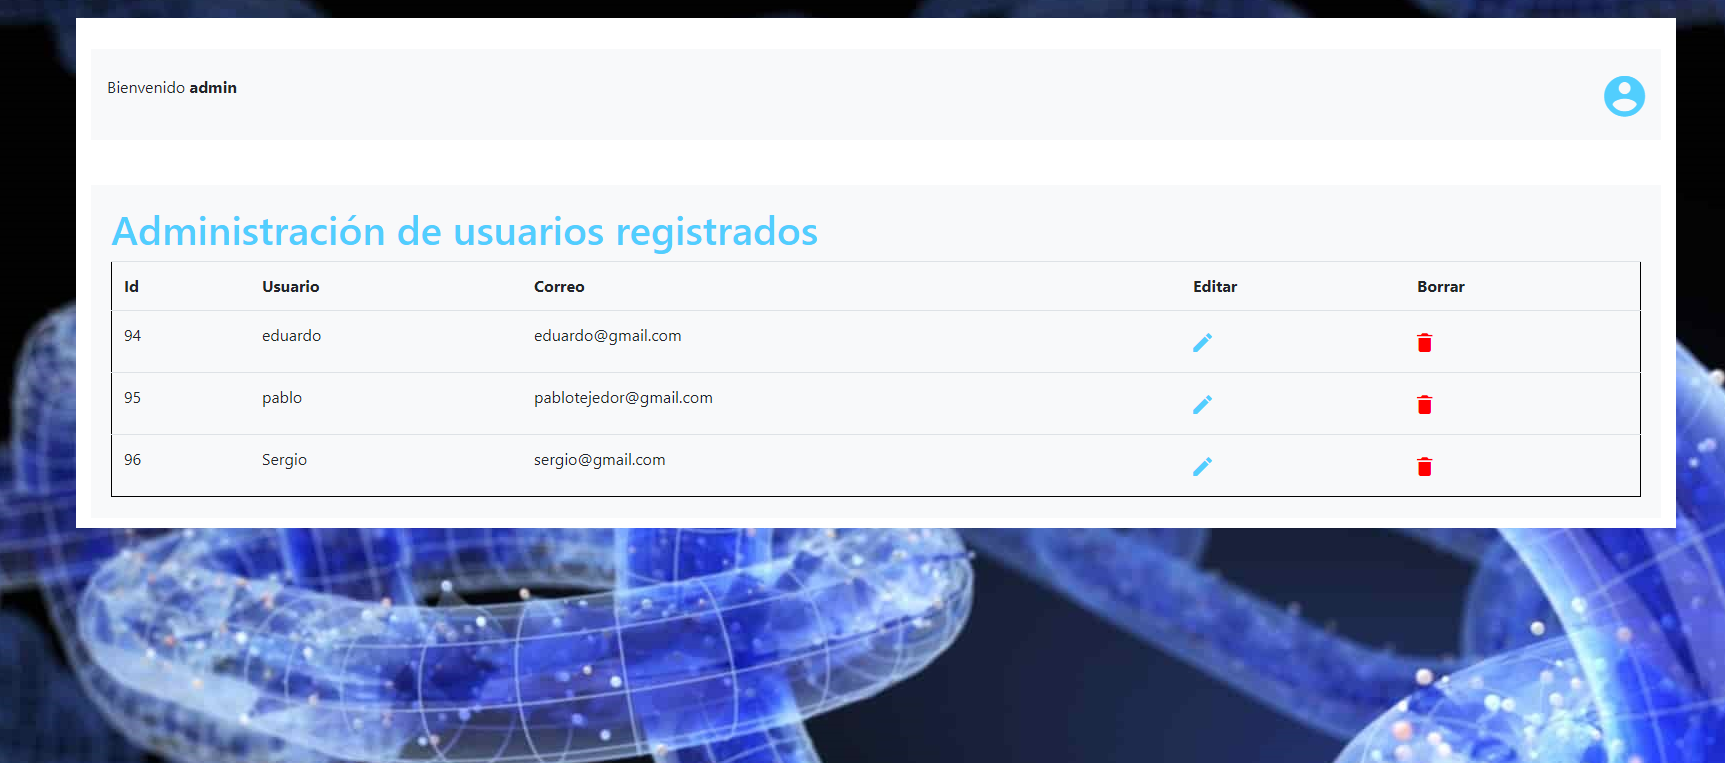
\includegraphics[width=\textwidth]{administrador}
    \caption{Administrador de usuarios}
    \label{fig:admin}
\end{figure}

El administrador será el responsable de poder gestionar y editar o borrar a los usuarios.

\paragraph{Administrador: \textit{Editar}} \ref{fig:editar}: en la cabecera nos informará mediante un mensaje de ``Bienvenido ...'' el usuario con el que se encuentra en cada momento. En la parte derecha tendremos un icono del avatar y en está pantalla nos permitirá cerrar sesión.

Si pulsamos en el lápiz azul de la columna editar de la fotografía \ref{fig:admin}  nos llevará a la siguiente pantalla:

 \begin{figure}[H]
    \centering
    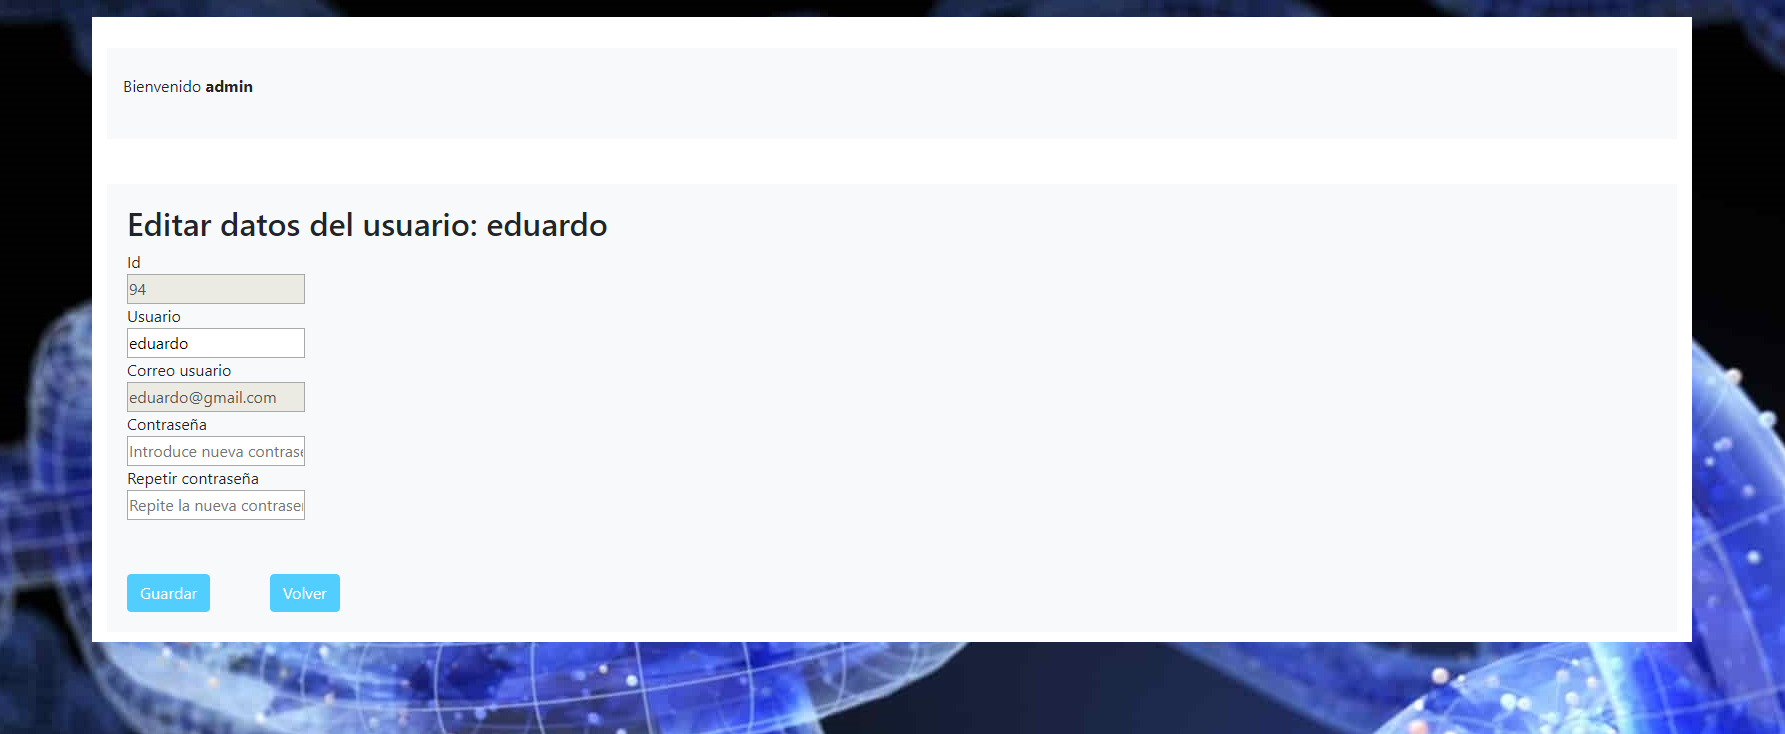
\includegraphics[width=\textwidth]{editarAdmin}
    \caption{Editar usuario desde administrador}
    \label{fig:editar}
\end{figure}

Nos mostrará los campos del usuario, pero únicamente podremos cambiar usuario y la contraseña, y nunca estos campos podrán quedar vacíos si hemos introducido algún valor anteriormente.

Cuando guardemos nos indicará si todo fue correcto, y, en caso de haber puesto las contraseñas incorrectas o el usuario vacío, nos mostrará un mensaje de error y tendremos que volver a realizar la misma operación, esta vez teniendo más cuidado y poniendo todo correctamente.

\paragraph{Administrador: \textit{Borrar}} \ref{fig:borrar}: así mismo, si queremos borrar tendremos que pulsar el icono de la papelera de la imágen \ref{fig:admin}, con esta acción nos mostrará un mensaje indicando si deseamos realizar la acción o no.

%\imagen{borrar2}{Borrar usuario desde administrador}
\begin{figure}[H]
	\centering
	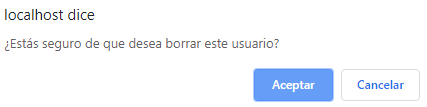
\includegraphics[width=0.7\textwidth]{confirmar}
	\caption{Mensaje confirmación}
	\label{fig:borrar}
\end{figure}

\paragraph{Opciones}\ref{fig:opciones}: una vez quedan explicadas las pantallas nos centramos en las que se involucran con el usuario de forma directa en su sesión.

Tendremos varias opciones en la pantalla de selección, los cuales explicaremos a continuación:
\begin{itemize}
	\item Añadir producto.
	\item Consultar el ultimo producto.
	\item Consultar todos los productos.
	\item Modificar datos (desde el avatar del usuario).
\end{itemize}

\begin{figure}[h!]
    \centering
    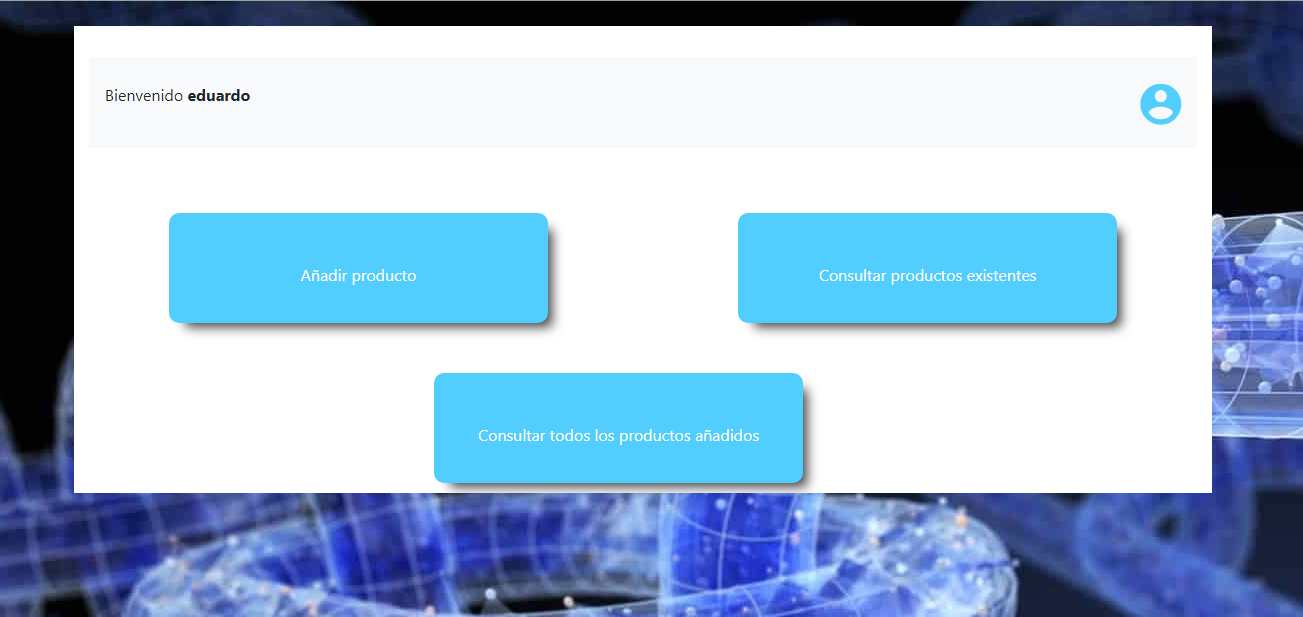
\includegraphics[width=0.7\textwidth]{opciones}
    \caption{Opciones a realizar por usuario}
    \label{fig:opciones}
\end{figure}

\paragraph{Añadir producto}: cuando pulsamos sobre la opción de añadir producto, esta automáticamente nos conectará con Metamask, pidiendo la contraseña \ref{fig:figura1e} (en caso de no estar logeados) o directamente nos dará la opción de conectar el proyecto con la cuenta que tengamos asociada de Metamask actualmente \ref{fig:figura2e}.

\begin{figure}[H]
	\begin{minipage}[b]{0.5\linewidth}
		\centering
		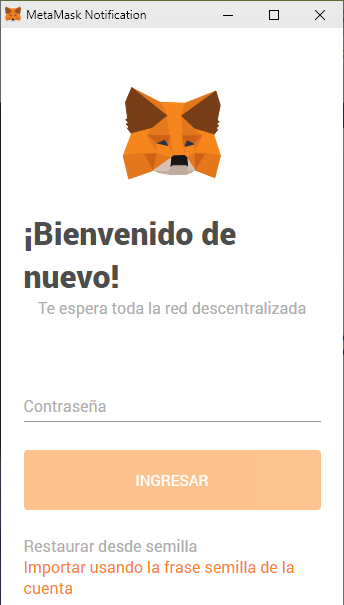
\includegraphics[width=\linewidth]{metamask-pantalla}
		\caption{Conexion Metamask}
		\label{fig:figura1e}
	\end{minipage}
	\hspace{0.5cm}
	\begin{minipage}[b]{0.5\linewidth}
		\centering
		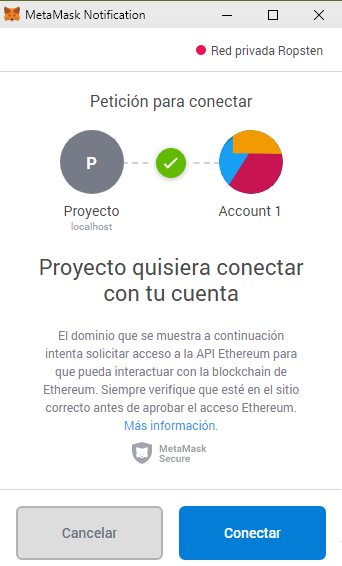
\includegraphics[width=\linewidth]{metamask-conexion}
		\caption{Conexion proyecto metamask}
		\label{fig:figura2e}
	\end{minipage}
\end{figure}

Una vez hemos completado el acceso y la conexión a metamask, tendremos que rellenar el producto que deseemos añadir \ref{fig:figura3e}, que serán los datos que almacenaremos en nuestro smart contract en la red Ethereum. 

\begin{figure}[H]
    \centering
    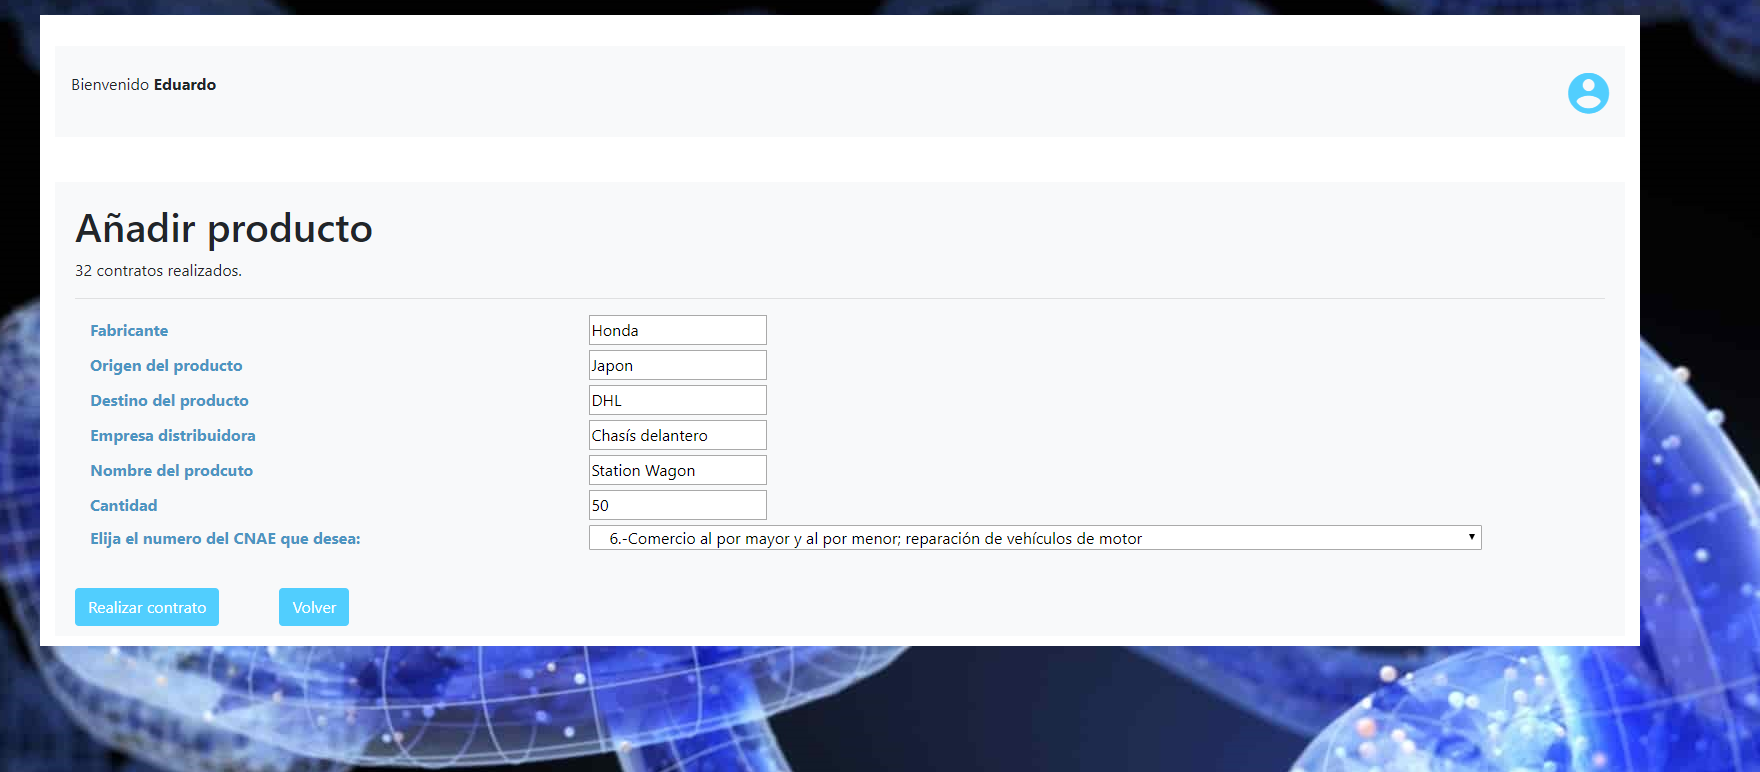
\includegraphics[width=1.00\textwidth]{anadirProdcuto1}
    \caption{Añadir producto}
    \label{fig:figura3e}
\end{figure}

Una vez rellenados los datos en nuestra pantalla, pulsaremos el botón de realizar contrato, esto nos mostrará nuevas pantallas que abrirá el conector de metamask para poder realizar el contrato \ref{fig:figura4e}, son las siguientes:

\begin{figure}[h!]
	\begin{minipage}[b]{0.5\linewidth}
		\centering
		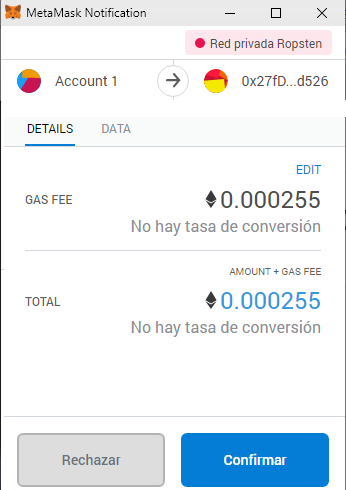
\includegraphics[width=\linewidth]{metamask-contrato}
		\caption{Confirmar el contrato}
		\label{fig:figura4e}
	\end{minipage}
\hspace{0.5cm}
	\begin{minipage}[b]{0.5\linewidth}
		\centering
		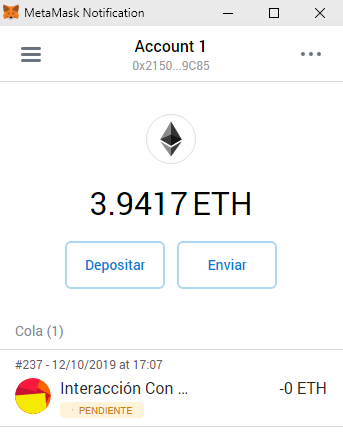
\includegraphics[width=\linewidth]{metamask-pendiente}
		\caption{Conexión pendiente}
		\label{fig:figura5e}
	\end{minipage}
	\begin{minipage}[b]{0.8\linewidth}
		\centering
		
\includegraphics[width=\linewidth]{metamask-cofnirmado}
		\caption{Conexión confirmada}
		\label{fig:figura6e}
	\end{minipage}
\end{figure}

Cuando el usuario realiza la acción de añadir un nuevo producto, antes de guardar todos los datos, primero se tiene que conectar con la red Ethereum, y hasta que no se crea el \textit{smart contract}, estos datos no quedarán debidamente guardados en la base de datos. 
 
Una vez que se haya confirmado la transacción \ref{fig:figura6e} en metamask, los datos se habrán guardado tanto en nuestra base de datos como en la red Ethereum de la red privada Ropsten. Si por un causal hubiera fallo de red o no tuviéramos conexión a la red, estos datos se perderían y tendríamos que realizar el contrato nuevamente para guardarlos. 

Para poder ver dicha transacción existen dos opciones: en la red Ethereum o bien mediante la nuestra página web.

En la red tendremos varias formas de llegar, pulsando directamente cuando nos sale el aviso de la \ref{fig:figura6e}, también se puede llegar pulsando en el icono de Metamask y la transacción que deseemos pulsar sobre la fecha ver en Etherscan. Una vez pulsado nos redirige a una pagina, llamada rospten.etherscan.io y el código de la transacción según cuál sea la que estamos trabajando.

En esta nueva pagina podremos ver toda la información del contrato mediante dos pestañas encontradas en la parte superior de la página:\hfill

\begin{itemize}
 \item  \textbf{Overview} \ref{fig:figura7e}: el estado y la hora de la transacción, la cuenta desde la que se hizo y a la cuenta que se realiza la transacción, el gas y el coste de ether. 
 
 \item \textbf{Event Logs} \ref{fig:figura8e}: en la cual podremos ver los datos que hemos introducido en nuestra pantalla de añadir producto(al principio nos saldrán todas los datos en formato hexadécimal y convertirlo a formato text o formato numérico según el datos que estemos buscando).
 \end{itemize}
 \begin{figure}[H]
    \centering
    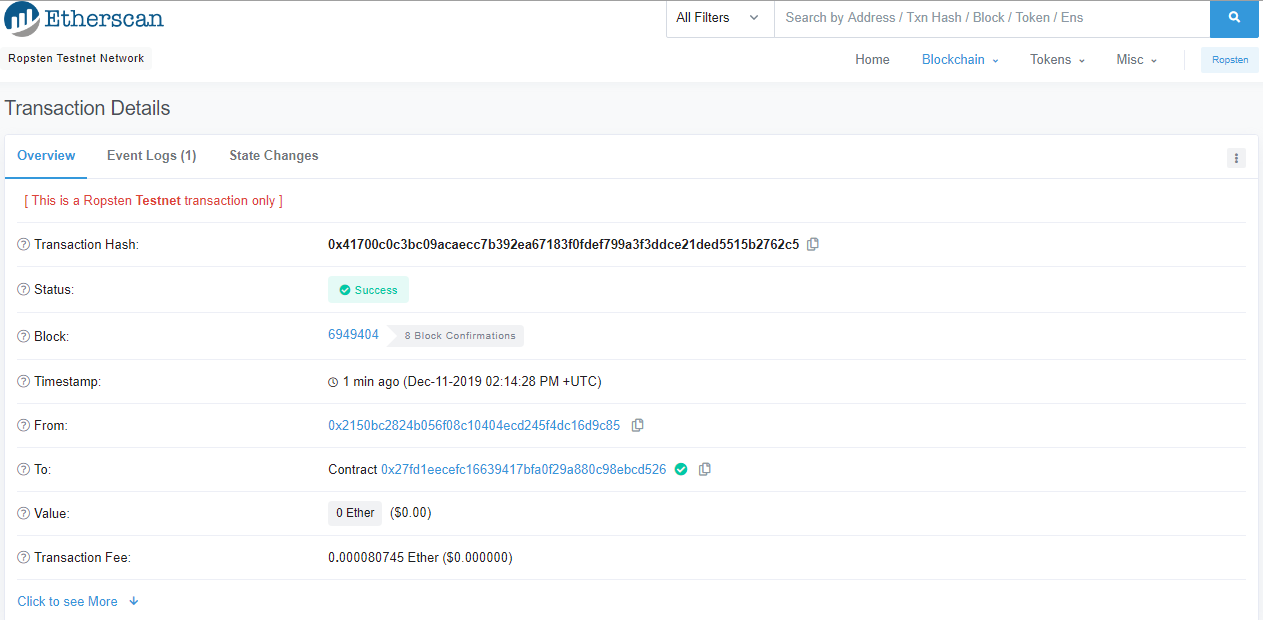
\includegraphics[width=\textwidth]{etherscan}
    \caption{Información del contrato creado vistos por Etherscan}
    \label{fig:figura7e}
\end{figure}
\begin{figure}[H]
    \centering
    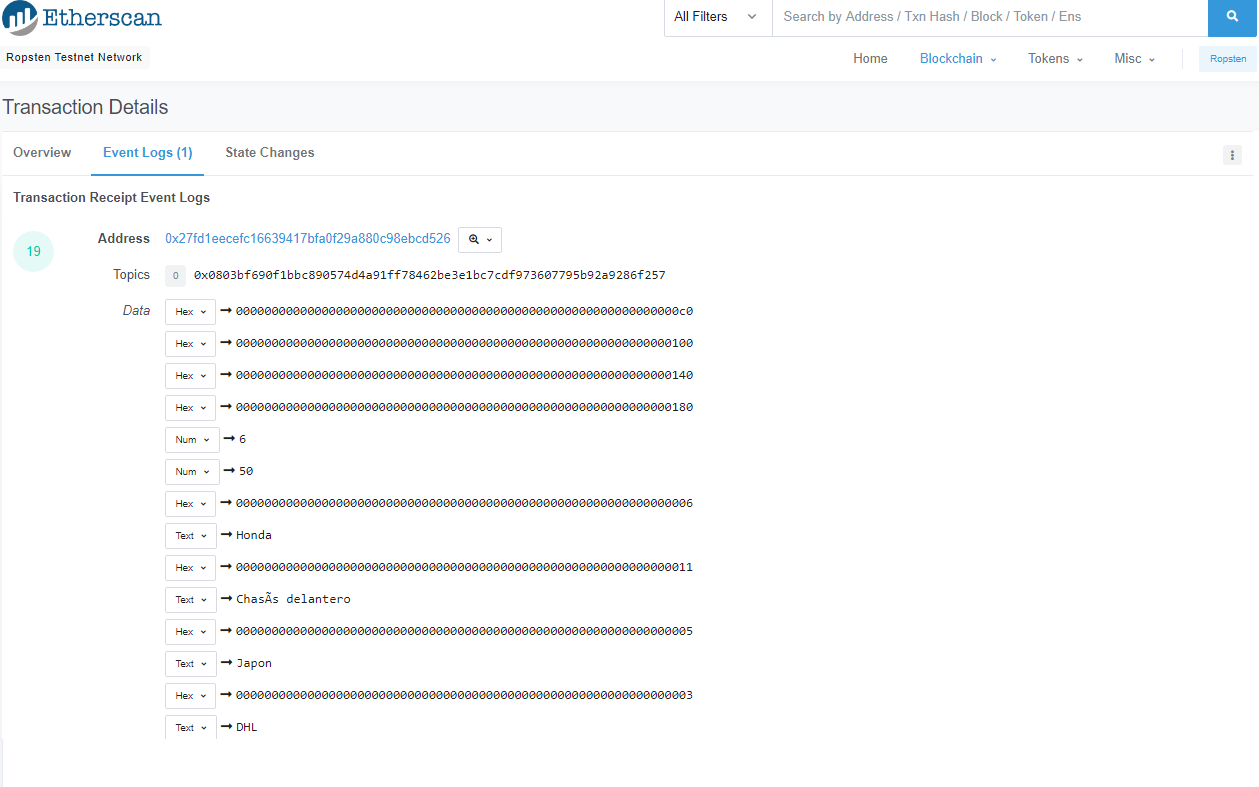
\includegraphics[width=\textwidth]{datos-etherscan}
    \caption{Datos proporcionados por Etherscan}
    \label{fig:figura8e}
\end{figure}


Una vez vistos todos estos datos en cuanto a la conexión de la red con Metamask y, esta a su vez, con la red Ropsten y Etherscan, ya tendríamos nuestro contrato ubicado en la red en todo momento, siempre que tengamos el enlace o bien la aplicación de metamask en la transacción que deseemos saber los datos.

\paragraph{Consultar todas las transacciones y la última transacción} \ref{fig:figura9e}: en el apartado anterior se explicó como observar la transacción que se realizó en un momento dado gracias a la red Etherscan. La otra forma de poder observarlas es dar a ``volver'', una vez confirmada la transacción. Lo que intentamos realizar con la creación de estos dos botones es que el usuario de la página no tenga que perder el tiempo entrando en esta red y poder buscarlo de forma más eficaz.

\begin{figure}[h!]
	\centering
	\begin{minipage}{0.8\linewidth}
		\centering
    	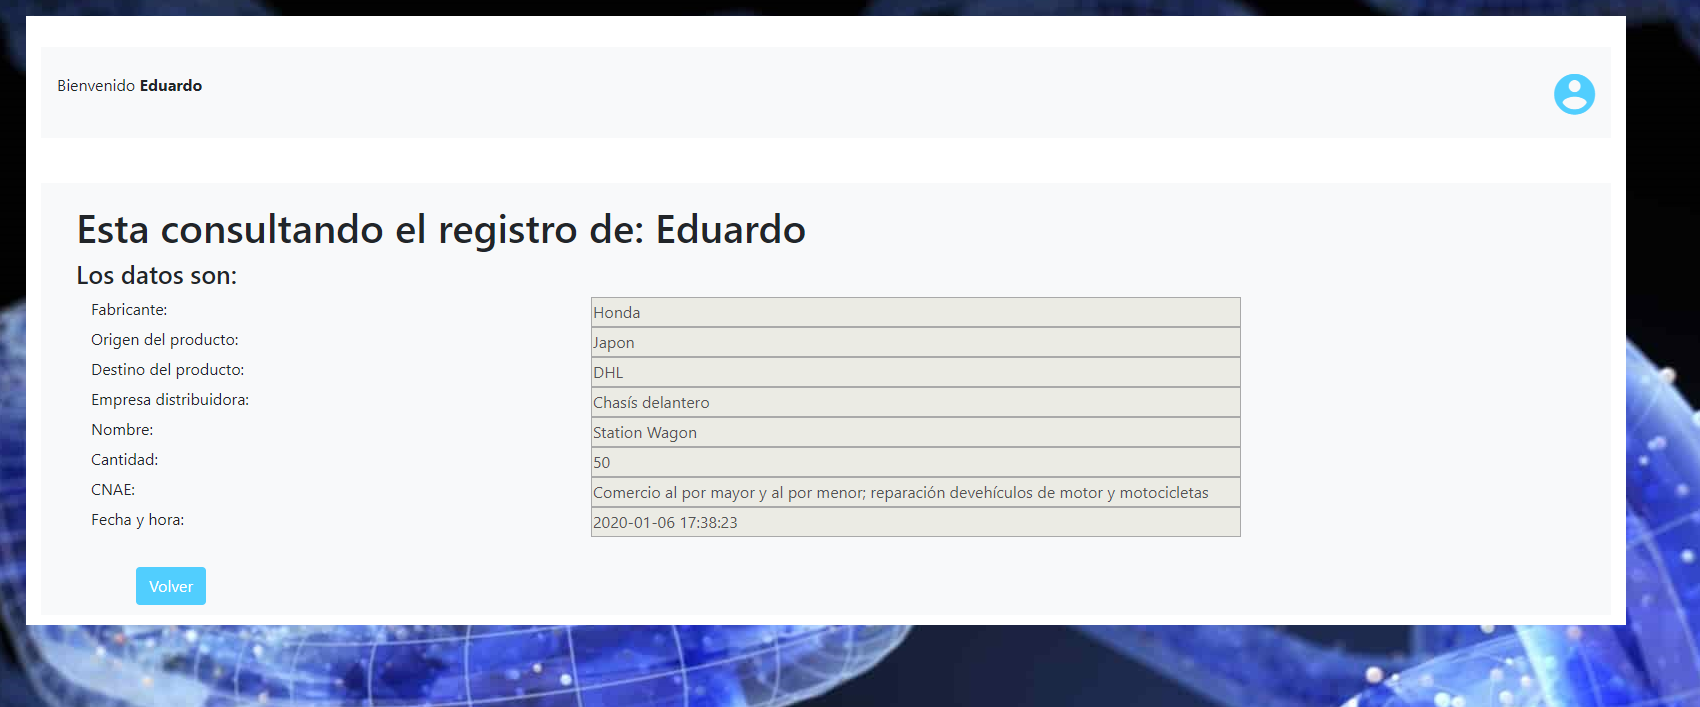
\includegraphics[width=\textwidth]{ultimoContrato}
    	\caption{Visualización del último producto}
    	\label{fig:figura9e}
	\end{minipage}
	\begin{minipage}{0.8\linewidth}
		 \centering
    	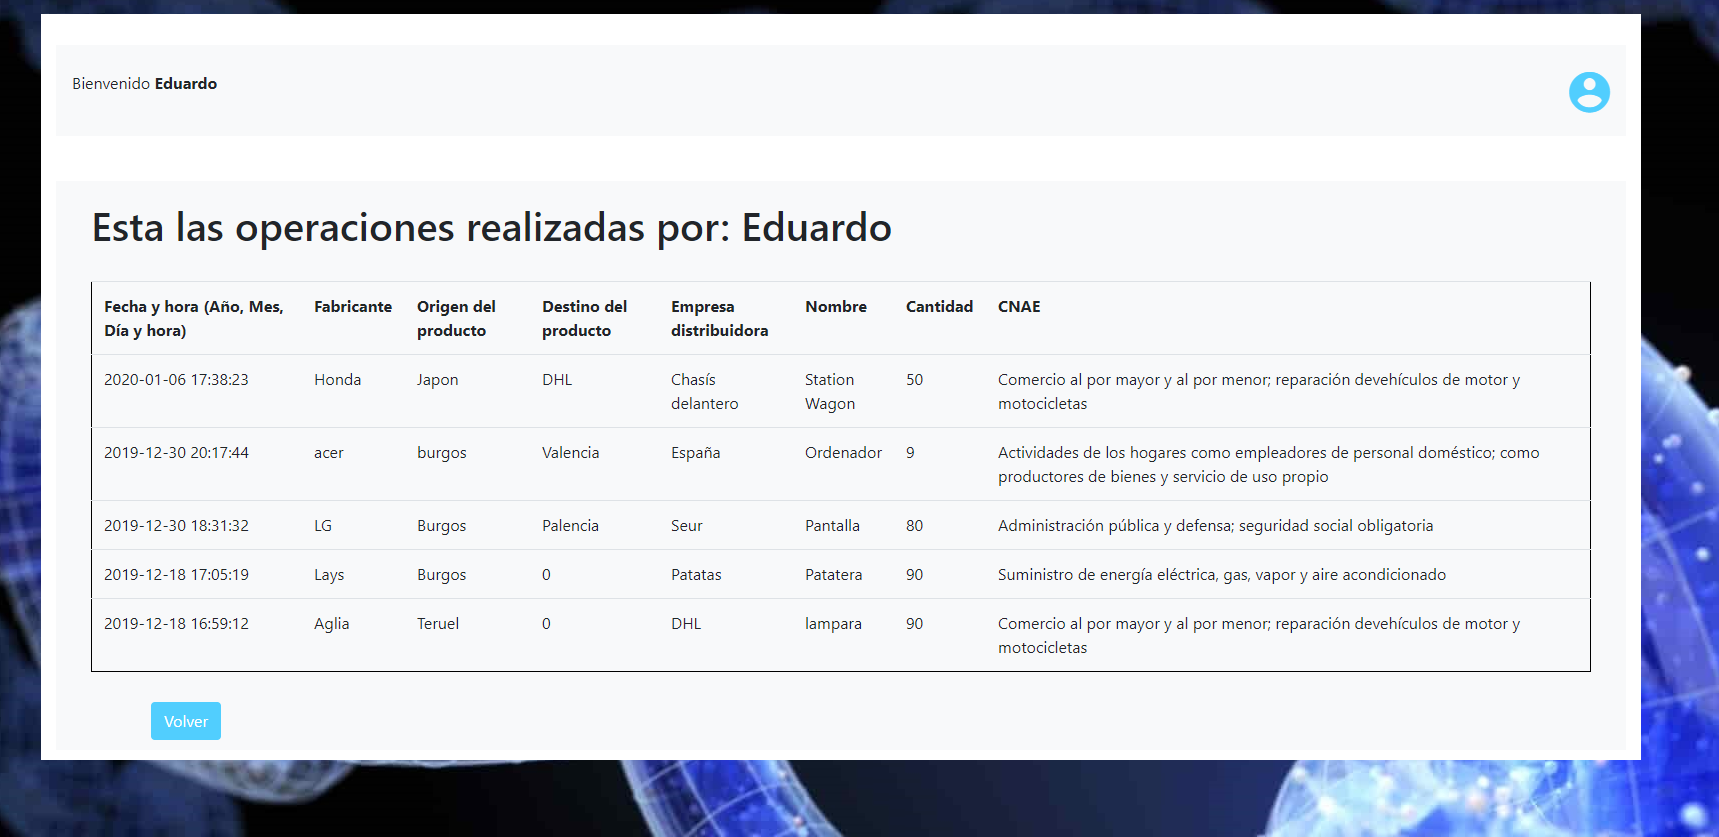
\includegraphics[width=\textwidth]{todosContratos}
    	\caption{Visualización de todos los productos realizados}
    	\label{fig:figura10e}
	\end{minipage}
\end{figure}

Las transacciones que realicemos nunca se podrán modificar ni borrar. Cierto es que en nuestra página (hemos decidido que mientras el usuario tenga una cuenta. Exista la transacción, pero si borramos al usuario, estaremos eliminado todos los contratos que creó de nuestra base de datos) pero en la red de Etherscan se podrán seguir visualizando de forma permanente, tal y como se explicó anteriormente. 


\bibliographystyle{plain}
\bibliography{bibliografiaAnexos}

\end{document}